\onehalfspacing

\allsectionsfont{\sffamily}
\newcommand{\ra}[1]{\renewcommand{\arraystretch}{#1}}

\let\Oldpart\part
\newcommand{\parttitle}{}
\renewcommand{\part}[1]{\Oldpart{#1}\renewcommand{\parttitle}{#1}}

\renewcommand{\chaptermark}[1]{\markboth{\textsf{Part \thepart.~ \parttitle}}{}}
\renewcommand{\sectionmark}[1]{\markright{\textsf{\thechapter.~ chapter title}}}

\hypertarget{acknowledgements}{%
\chapter*{Acknowledgements}\label{acknowledgements}}
\addcontentsline{toc}{chapter}{Acknowledgements}

\hypertarget{summary}{%
\chapter*{Summary}\label{summary}}
\addcontentsline{toc}{chapter}{Summary}

\hypertarget{samenvatting}{%
\chapter*{Samenvatting}\label{samenvatting}}
\addcontentsline{toc}{chapter}{Samenvatting}

\hypertarget{list-of-publications}{%
\chapter*{List of publications}\label{list-of-publications}}
\addcontentsline{toc}{chapter}{List of publications}

\hypertarget{list-of-conferences}{%
\chapter*{List of conferences}\label{list-of-conferences}}
\addcontentsline{toc}{chapter}{List of conferences}

\mainmatter

\hypertarget{introduction}{%
\chapter{Introduction}\label{introduction}}

\hypertarget{unipept-desktop}{%
\part{Unipept Desktop}\label{unipept-desktop}}

The introductory text for this part comes here\ldots{}

\hypertarget{unipept-desktop-a-faster-more-powerful-metaproteomics-analysis-tool}{%
\chapter{Unipept Desktop: a faster, more powerful metaproteomics
analysis
tool}\label{unipept-desktop-a-faster-more-powerful-metaproteomics-analysis-tool}}

\markright{\textsf{High-throughput metaproteomics analysis}}

\textbf{Abstract} Metaproteomics has become an important research tool
to study microbial systems, which has resulted in increased
metaproteomics data generation. However, efficient tools for processing
the acquired data have lagged behind. One widely used tool for
metaproteomics data interpretation is Unipept, a web-based tool that
provides, amongst others, interactive and insightful visualizations. Due
to its web-based implementation, however, the Unipept web application is
limited in the amount of data that can be analyzed. In this manuscript
we therefore present Unipept Desktop, a desktop application version of
Unipept that is designed to drastically increase the throughput and
capacity of metaproteomics data analysis. Moreover, it provides a novel
comparative analysis pipeline and improves the organization of
experimental data into projects, thus addressing the growing need for
more performant and versatile analysis tools for metaproteomics data.

\hypertarget{introduction-1}{%
\section{Introduction}\label{introduction-1}}

Metaproteomics is a relatively young research field that focuses on the
study of microbial environments and complex ecosystems, and of the
interactions between the organisms involved, through the analysis of the
proteins extracted from these environments. Over the past years, the
technology to identify proteins from such complex samples has been
greatly improved, allowing metaproteomics to transition from relatively
small studies to large scale experiments (Rechenberger \emph{et al.},
2019; Wilmes \emph{et al.}, 2015). The key enabling technologies for
this transition are improved mass spectrometers and more powerful
proteomics approaches, which have both come a long way since the
introduction of metaproteomics analysis in 2004 (Rodríguez-Valera, 2004;
Yates, 2019). To allow efficient processing of the resulting increase of
acquired data, various dedicated tools have been made available to
support metaproteomics data analysis (Muth \emph{et al.}, 2015; Van Den
Bossche \emph{et al.}, 2020), but even with this increased
bioinformatics support, many challenges still need to be overcome,
especially regarding downstream analysis of the obtained identifications
(Schiebenhoefer \emph{et al.}, 2019).

Unipept is a leading tool for such downstream metaproteomics data
analysis (Herbst \emph{et al.}, 2016) that currently consists of a web
application (Gurdeep Singh \emph{et al.}, 2019), a web service, and a
command line tool (Verschaffelt \emph{et al.}, 2020). The Unipept web
application provides users with the ability to analyze a metaproteomics
sample and extract taxonomic and functional information from
environmental samples derived from a variety of origins, ranging from
the human gut to biogas plants. The Unipept web application provides
users with interactive visualizations and allows them to, for example,
filter out all functions that are associated with a specific taxon. Due
to its web-based nature, however, the size and number of samples that
can be analyzed by Unipept are limited. And while it is currently
possible to analyze larger data sets using the Unipept CLI, this
requires more sophisticated bioinformatics skills and does not provide
the interactive link between taxa and functional annotations.

Because of the browser limitations, it can already take a substantial
amount of time to process relatively small samples (e.g.~containing up
to a few thousand identified peptides) using Unipept, depending on the
specific search configuration used. These limitations have become an
issue, as the advances in metaproteomics have not only increased data
set sizes, but have also increased the number of data sets that need to
be processed (Zhang and Figeys, 2019).

In order to accommodate this evolution, the throughput of metaproteomics
data analyses needs to increase as well, in turn requiring tools that
are not constrained in the amount of memory and CPU resources they are
allowed to consume. Moreover, analysis results also need to be retained
for future reference, ideally in a project-based approach that can group
multiple samples, and the corresponding results should be easily
shareable with other researchers.

For specific applications, it is also important that all data is
processed offline or on-site rather than being sent over the internet.
For instance, sensitive medical data is often not allowed to be sent to
external services for processing, but must be kept in-house to safeguard
patient confidentiality and privacy.

All of the above issues need to be resolved in order to support the
growing interest in, and reach of, metaproteomics. We therefore here
present the Unipept Desktop Application, a novel cross-platform desktop
application designed to specifically overcome these challenges while
also retaining the functionality that exists in the current web app.

\hypertarget{implementation}{%
\section{Implementation}\label{implementation}}

\begin{figure}
\centering
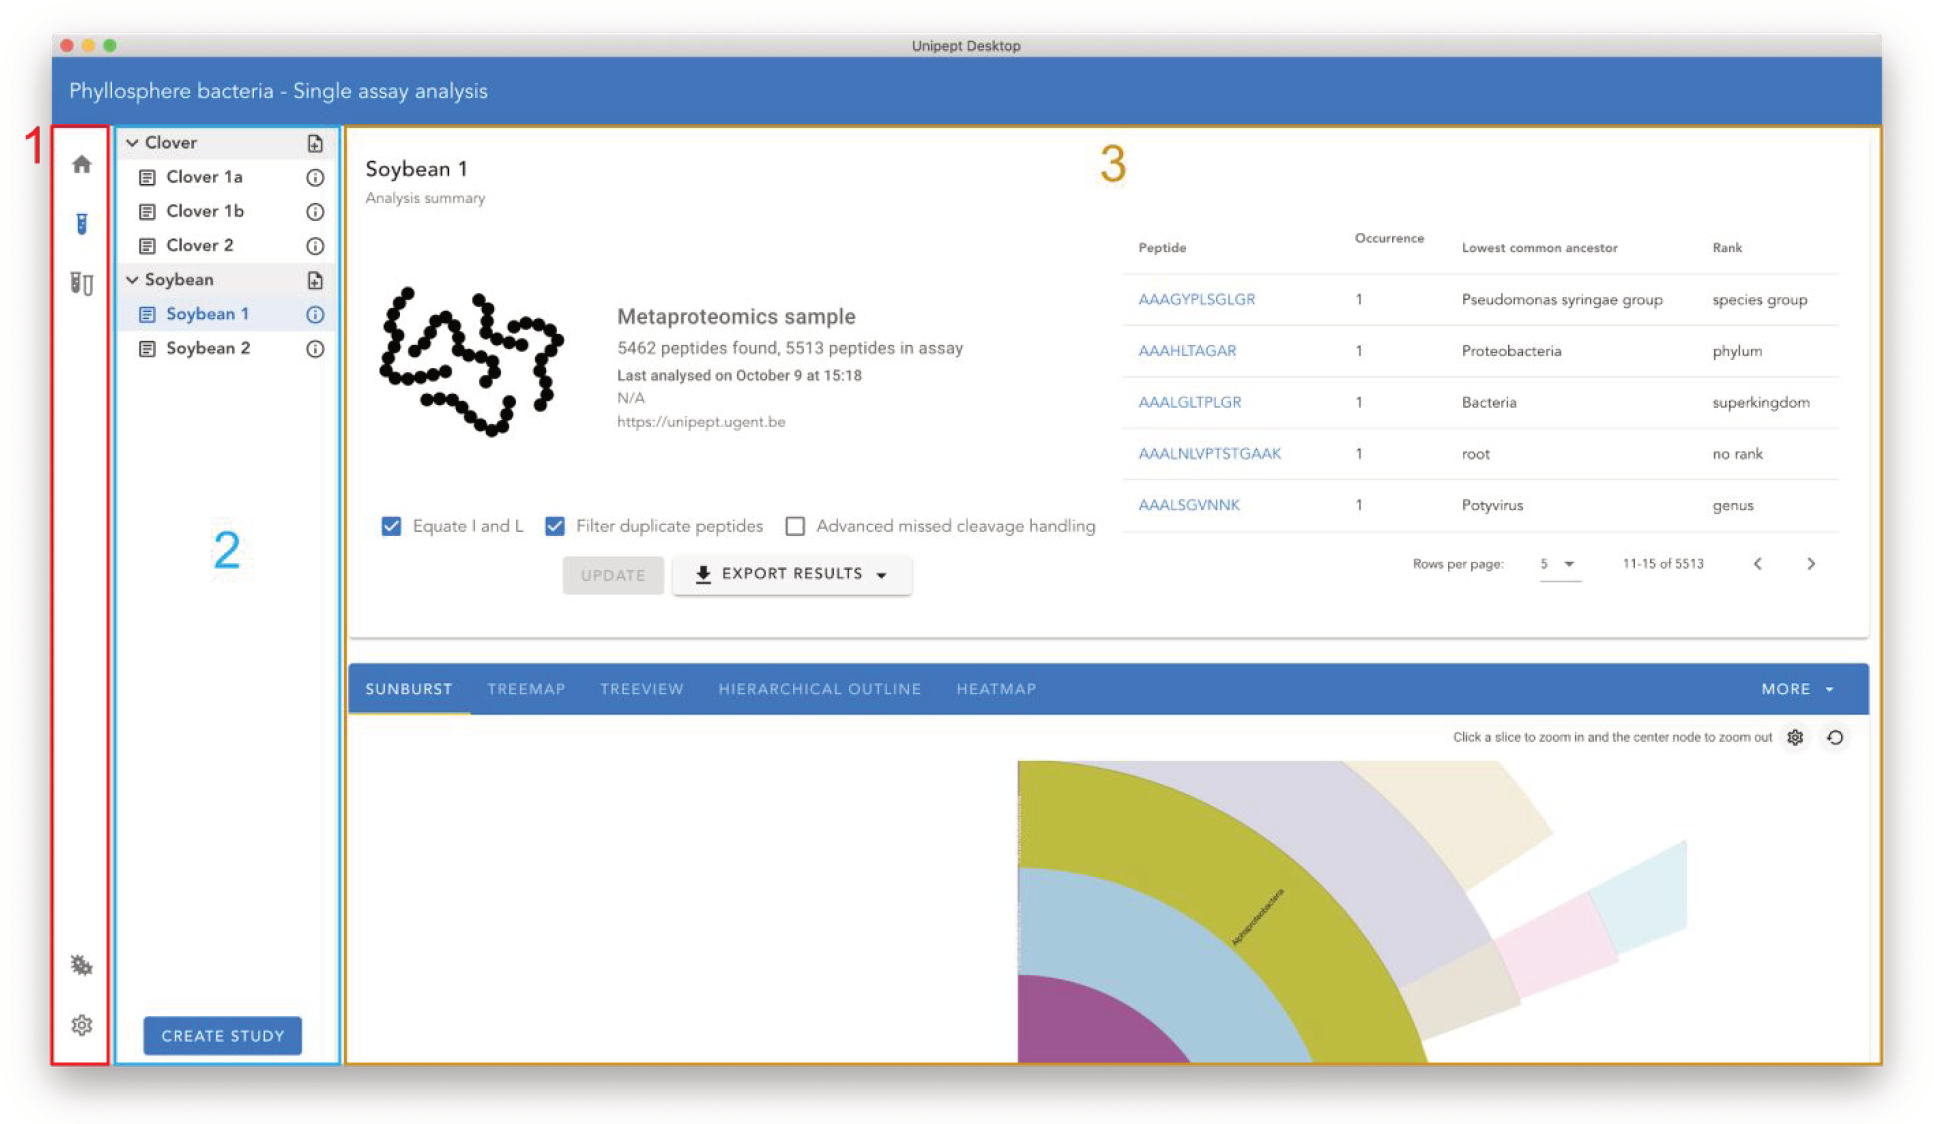
\includegraphics{resources/figures/chapter2_application_overview_screenshot.png}
\caption{Screenshot of the Unipept Desktop application. The analysis
page of the desktop application is depicted here and consists of three
main parts: the sidebar that is used to navigate between the different
analysis pipelines and functions of the application (1), the project
explorer that displays a hierarchical view of the project (2) and the
content view that renders analysis results
(3).\label{fig:desktop_app_overview_screenshot}}
\end{figure}

The Unipept desktop application provides three different types of
analyses: \emph{i}) single assay analysis, \emph{ii}) inter-assay
comparative analysis, and \emph{iii}) tryptic peptide analysis. The
single assay analysis performs a full taxonomic and functional analysis
of a single assay and corresponds to the default ``metaproteomics
analysis'' as presented by the Unipept web application. The inter-assay
comparative analysis on the other hand, provides the ability to explore
similarities and differences between multiple assays. While the
comparison of multiple assays was already possible with the Unipept web
application, this was only available for a limited number of quite small
assays due to strict memory constraints posed by web browsers. The
tryptic peptide analysis, lastly, can be used to look up which proteins,
taxa and functions are associated with a given peptide.

Unipept Desktop delivers these core functions through a concise user
interface (\autoref{fig:desktop_app_overview_screenshot}) that consists
of three main parts: the sidebar, the project explorer, and the content
view. The sidebar on the far left allows the user to navigate between
the different analysis pipelines and functions of this application.
Directly to the right of the sidebar is the project explorer that allows
the user to switch between assays, and to modify the project. The
project explorer is only shown when performing single assay or
comparative analyses. Assays and studies can be renamed or deleted by
right clicking them, after which a context menu opens. Lastly, the
content view takes up most of the application's visual space and
presents either analysis results or the settings page.

The Unipept Desktop Application also allows offline analysis of data
through a choice of the API endpoint in the settings menu. This
endpoint, which uses the Unipept API and by default connects to the
online Unipept system, can be configured to call any service that
supports the Unipept API. By setting up a local instance of the Unipept
backend system, the user can thus ensure that all data remains locally.
Setting up a local Unipept back-end is possible by cloning the open
source Unipept repository on GitHub, but requires advanced technical
knowledge. We plan to make the installation process of these custom API
endpoints even easier with future releases of Unipept.

Unipept Desktop is powered by the cross-platform Electron framework,
which in itself is powered by Chromium browser technology. This means
that the application is developed with web-centric technologies, such as
the Vue frontend framework and TypeScript, and hence we were able to
reuse large parts of the web app's codebase. The choice for the Electron
platform was mostly driven by the extensive suite of different
functionalities that can be integrated with minimum configuration
efforts. Thanks to the Electron platform we can provide an automatic
update mechanism, easily generate installation packages for all major
platforms (Windows, macOS and Linux), and include automatic crash
reporting, amongst others. Once installed, the Unipept Desktop
application can thus update fully autonomously in the background,
ensuring that users always have the latest functionality and bug fixes
installed.

\hypertarget{project-centric-analysis}{%
\subsection{Project-centric analysis}\label{project-centric-analysis}}

The Unipept Desktop Application has full access to the local filesystem.
Hence, it can store an arbitrary amount of data and does not need to
worry about strict size limits; this in contrast to web applications
that are only allowed to store up to a few megabytes using the local
storage API. This allows us to improve upon the organization of data
sets by introducing project-based data management capabilities. In
accordance with the terminology introduced by the ISA-tab standard for
experimental metadata annotation (Sansone \emph{et al.}, 2012), we now
refer to a data set derived from a sample as an ``assay'', while a study
is a grouping of multiple, related assays, and a Unipept project
represents a collection of such studies.

On the file system, a project is stored in a single folder that contains
an SQLite database file, a subfolder for each study and one text file
per assay, located in the subfolder of the corresponding study. This
folder can be modified outside of the application, using the default
file explorer application of your operating system, thus providing
maximum flexibility. All changes made to this project folder are
automatically detected and imported by the application, granting users
the ability to mass import assays and edit project properties with
external applications. The application accepts simple text files with
one peptide per line. In order to quantify peptide occurrence, a peptide
can be included more than once in this file and the ``filter duplicate
peptides'' option should be disabled for the analysis.

Because projects are folder-based, they can contain both the raw input
data as well as the analysis results for an assay, making it practical
for users to share projects with each other, for instance, in the form
of compressed project folders. In addition, previously performed
analyses do not need to be recomputed when the application is restarted,
as opposed to analyses that were run on the Unipept website, which need
to be recomputed every time the website is closed.

\hypertarget{comparative-analysis}{%
\subsection{Comparative analysis}\label{comparative-analysis}}

\begin{figure}
\centering
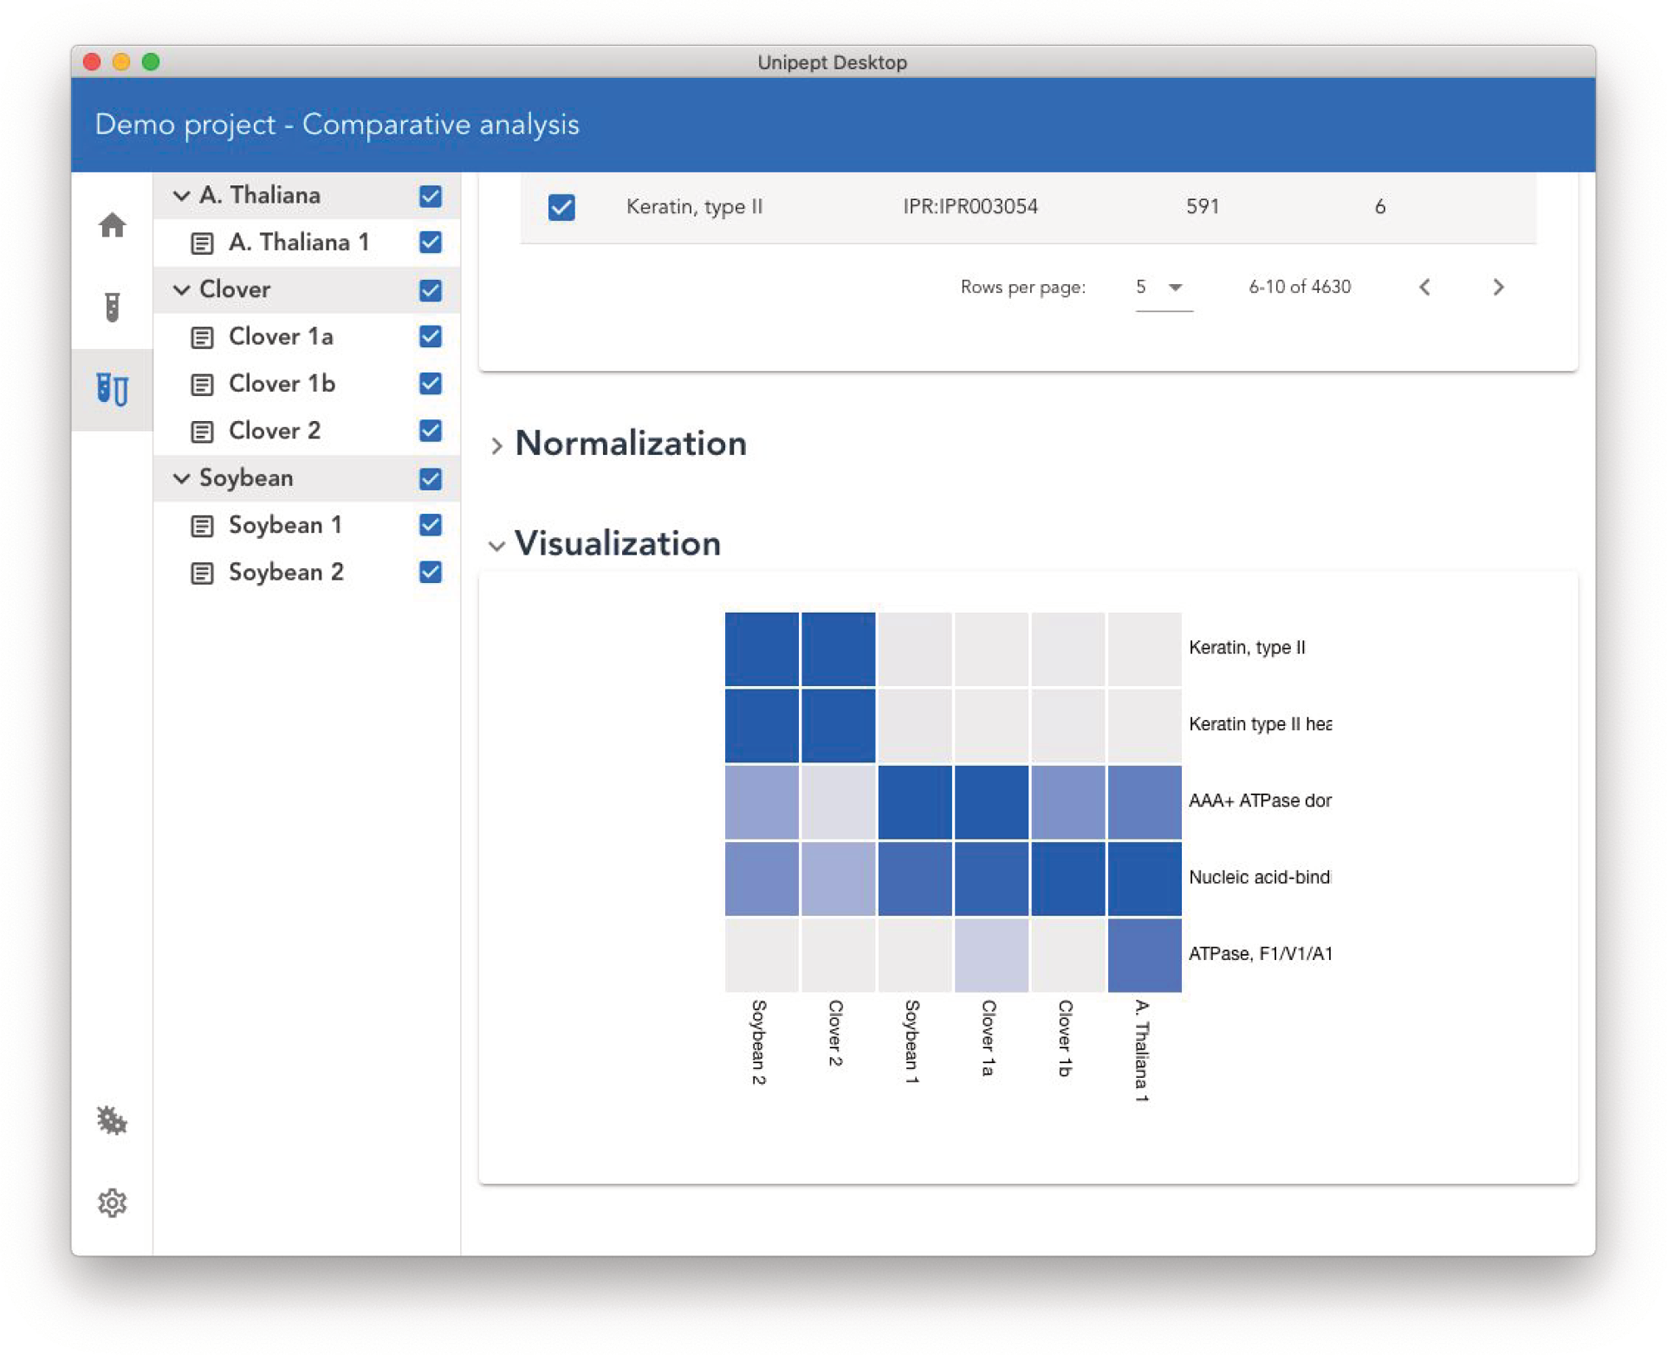
\includegraphics{resources/figures/chapter2_comparative_analysis_screenshot.png}
\caption{Screenshot of the inter-assay comparative analysis pipeline.
Note that it is possible to select multiple assays from the project
explorer. A heatmap is constructed from the set of items that were
selected for comparison at the top of the page.}
\end{figure}

The Unipept Desktop Application provides both intra-assay and
inter-assay comparative analyses that are rendered as heatmap
visualizations. The intra-assay comparison can be started from the
single assay analysis page by selecting the heatmap tab and provides a
wizard to guide users through the set-up process of the comparison
(Figure 2). Users are required to select two types of data sources (one
for each axis of the heatmap) and indicate which items should be
compared. Four different data sources are currently supported: NCBI
taxa, GO terms (The~Gene~Ontology~Consortium, 2019), EC numbers and
InterPro entries (Finn \emph{et al.}, 2017).

The inter-assay comparative analysis is designed to visualize
differences and similarities in functional or taxonomic composition of
multiple assays. Here too, users are presented with a wizard that is
similar to the one found in the intra-assay comparison. For inter-assay
comparisons, however, the horizontal axis of the heatmap is reserved for
the set of selected assays, and users can therefore only select one
collection of items that should be compared between the different
assays.

Because the number of peptides can drastically differ between multiple
assays, three different normalization techniques are provided to the
user. The default setting normalizes the heatmap globally, i.e.~the
minimum and maximum values over the complete grid are computed and all
grid values are normalized with respect to these values. The other two
normalization techniques also normalize based on minimum and maximum
values, but restricted within a row or column, respectively.

It is worth noting that, while the comparative analysis pipeline was
originally designed for the Unipept Desktop Application, a slimmed-down
version has meanwhile also been integrated into the Unipept web app.

With the advent of the Unipept Desktop Application, users now have a
variety of ways in which they can use Unipept. A comparison between the
various functionalities offered by these different services is provided
in \autoref{tab:comparison_of_unipept_services}.

\begin{table*}\centering
\renewcommand{\arraystretch}{1.3}
\begin{tabular}{@{}p{45mm}cccc@{}}\toprule
& desktop app & web app & CLI & API\\ \midrule
visualizations & \Checkmark & \Checkmark & $\sim$ & $\sim$ \\
basic metaproteomics analysis pipeline & \Checkmark & \Checkmark & \XSolidBrush & \XSolidBrush \\
tryptic peptide analysis pipeline & \Checkmark & \Checkmark & \XSolidBrush & \XSolidBrush \\
comparative analysis & \Checkmark & $\sim$ & \XSolidBrush & \XSolidBrush \\
metadata or projects & \Checkmark & \XSolidBrush & \XSolidBrush & \XSolidBrush \\
custom endpoint & \Checkmark & \XSolidBrush & \Checkmark & \XSolidBrush \\
store analysis results & \Checkmark & \XSolidBrush & $\sim$ & \XSolidBrush \\
process large samples & \Checkmark & \XSolidBrush & \Checkmark & \Checkmark \\
no command line knowledge required & \Checkmark & \Checkmark & \XSolidBrush & \XSolidBrush \\
no installation required & \XSolidBrush & \Checkmark & \XSolidBrush & \Checkmark \\
\bottomrule
\end{tabular}
\caption{Comparison of the functionalities provided by the different Unipept services. \label{tab:comparison_of_unipept_services}}
\end{table*}

\hypertarget{conclusion}{%
\section{Conclusion}\label{conclusion}}

Unipept Desktop is a novel desktop application that extends upon the
Unipept web application by eradicating the strict limitations posed by
the web-based nature of this application to increase metaproteomics data
analysis throughput. Moreover, the Unipept Desktop Application adds new
features such as allowing users to structure their data in a
hierarchical project-based system, to keep track of their analysis
results, and to share or distribute these results very easily. Whereas
the Unipept web application is limited to assays with up to 50 000
peptides, the Unipept Desktop Application supports assays containing one
million peptides or more. For reference, the desktop app can analyze
between 250 and 2000 peptides per second (without advanced missed
cleavage handling enabled), depending on the type of assay that's being
analyzed.

In a future release of the Unipept Desktop Application, we plan to
provide support for the preparation of custom reference databases and
further improve support for offline analysis. This will allow us to
gradually evolve to a tool that is not only suitable for metaproteomics
data analysis, but also for novel proteogenomics analysis techniques for
complex environmental samples.

Our choice for the Electron framework proves to be very valuable as
well, as a large portion of Unipept's codebase can thus be shared
between the new desktop application and the existing web application.
This in turn allows us to easily migrate (a slimmed-down version of)
specific desktop features to the web app, and vice versa.

\hypertarget{availability}{%
\section{Availability}\label{availability}}

The source code for Unipept Desktop is open source and provided under
the MIT license as a repository on GitHub:
\url{https://github.com/unipept/unipept-desktop}. Pre-generated
installers for Windows, macOS and Linux (AppImage format) can be
downloaded from the release page of our GitHub repository. Installation
instructions and documentation for the Unipept Desktop Application can
be found on our website: \url{https://unipept.ugent.be/desktop}.

\hypertarget{acknowledgements-1}{%
\section{Acknowledgements}\label{acknowledgements-1}}

This work was supported by the Research Foundation---Flanders (FWO)
{[}1164420N to P.V.; 12I5220N to B.M.; 1S90918N to T.V.D.B.; G042518N to
L.M. {]}.

\newpage

\hypertarget{support-for-novel-proteogenomics-analysis-in-unipept}{%
\chapter{Support for novel proteogenomics analysis in
Unipept}\label{support-for-novel-proteogenomics-analysis-in-unipept}}

\markright{Support for proteogenomics analyses}

\hypertarget{other-projects}{%
\part{Other projects}\label{other-projects}}

The introductory text for this chapter comes here\ldots{}

\hypertarget{megago-a-fast-yet-powerful-approach-to-assess-functional-gene-ontology-similarity-across-meta-omics-data-sets}{%
\chapter{MegaGO: a fast yet powerful approach to assess functional Gene
Ontology similarity across meta-omics data
sets}\label{megago-a-fast-yet-powerful-approach-to-assess-functional-gene-ontology-similarity-across-meta-omics-data-sets}}

\markright{\textsf{A new similarity metric for comparing sets of GO-terms}}

\textbf{Abstract} The study of microbiomes has gained in importance over
the past few years and has led to the emergence of the fields of
metagenomics, metatranscriptomics, and metaproteomics. While initially
focused on the study of biodiversity within these communities, the
emphasis has increasingly shifted to the study of (changes in) the
complete set of functions available in these communities. A key tool to
study this functional complement of a microbiome is Gene Ontology (GO)
term analysis. However, comparing large sets of GO terms is not an easy
task due to the deeply branched nature of GO, which limits the utility
of exact term matching. To solve this problem, we here present MegaGO, a
user-friendly tool that relies on semantic similarity between GO terms
to compute the functional similarity between multiple data sets. MegaGO
is high performing: Each set can contain thousands of GO terms, and
results are calculated in a matter of seconds. MegaGO is available as a
web application at \url{https://megago.ugent.be} and is installable via
pip as a standalone command line tool and reusable software library. All
code is open source under the MIT license and is available at
\url{https://github.com/MEGA-GO/}.

\hypertarget{introduction-2}{%
\section{Introduction}\label{introduction-2}}

Microorganisms often live together in a microbial community or
microbiome where they create complex functional networks. These
microbiomes are therefore commonly studied to reveal both their
taxonomic composition as well as their functional repertoire. This is
typically achieved by analyzing their gene content using shotgun
metagenomics. Whereas this approach allows a detailed investigation of
the genomes that are present in such multiorganism samples, it reveals
only their functional potential rather than their currently active
functions (Jansson and Baker, 2016). To uncover these active functions
within a given sample, the characterization of the protein content is
often essential (Lohmann \emph{et al.}, 2020).

The growing focus on functional information as a complement to taxonomic
information (Louca \emph{et al.}, 2016) is derived from the observation
that two taxonomically similar microbial communities could have vastly
different functional capacities, whereas taxonomically quite distinct
communities could have remarkably similar functions. Whereas the
investigation of the active functions is thus increasingly seen as vital
to a complete understanding of a microbiome, the identification and
comparison of these detected functions remains one of the biggest
challenges in the field (Schiebenhoefer \emph{et al.}, 2019).

Several omics tools exist to describe functions in microbial samples,
although these tools link functionality to different biological entities
such as genes, transcripts, proteins, and peptides (Muth \emph{et al.},
2015, 2018; Van Den Bossche \emph{et al.}, 2020; Verschaffelt \emph{et
al.}, 2020; Gurdeep Singh \emph{et al.}, 2019; Riffle \emph{et al.},
2018; Schneider \emph{et al.}, 2011; Schiebenhoefer \emph{et al.}, 2020;
Huerta-Cepas \emph{et al.}, 2019; Huson \emph{et al.}, 2007). However,
most tools are capable of directly or indirectly reporting functional
annotations as a set of Gene Ontology (The~Gene~Ontology~Consortium,
2019) (GO) terms, regardless of the biological entities they are
assigned to. In October 2020, there were 44264 of these terms in the
complete GO tree. GO terms are organized into three independent domains:
molecular function, biological process, and cellular component
(Ashburner \emph{et al.}, 2000). In each domain, terms are linked into a
directed acyclic graph, an excerpt of which is shown in
\autoref{fig:megago_biological_process_excerpt}. In the GO graph, a
parent term can have one or more child (e.g., the root node ``biological
process'' is the parent of the children GO:0009987 and GO:0008152), and
children can have multiple parents (e.g., the most specific term
``translation'' has GO:0043043, GO:0034645, and GO:0044267 as parents).

\begin{figure}
\centering
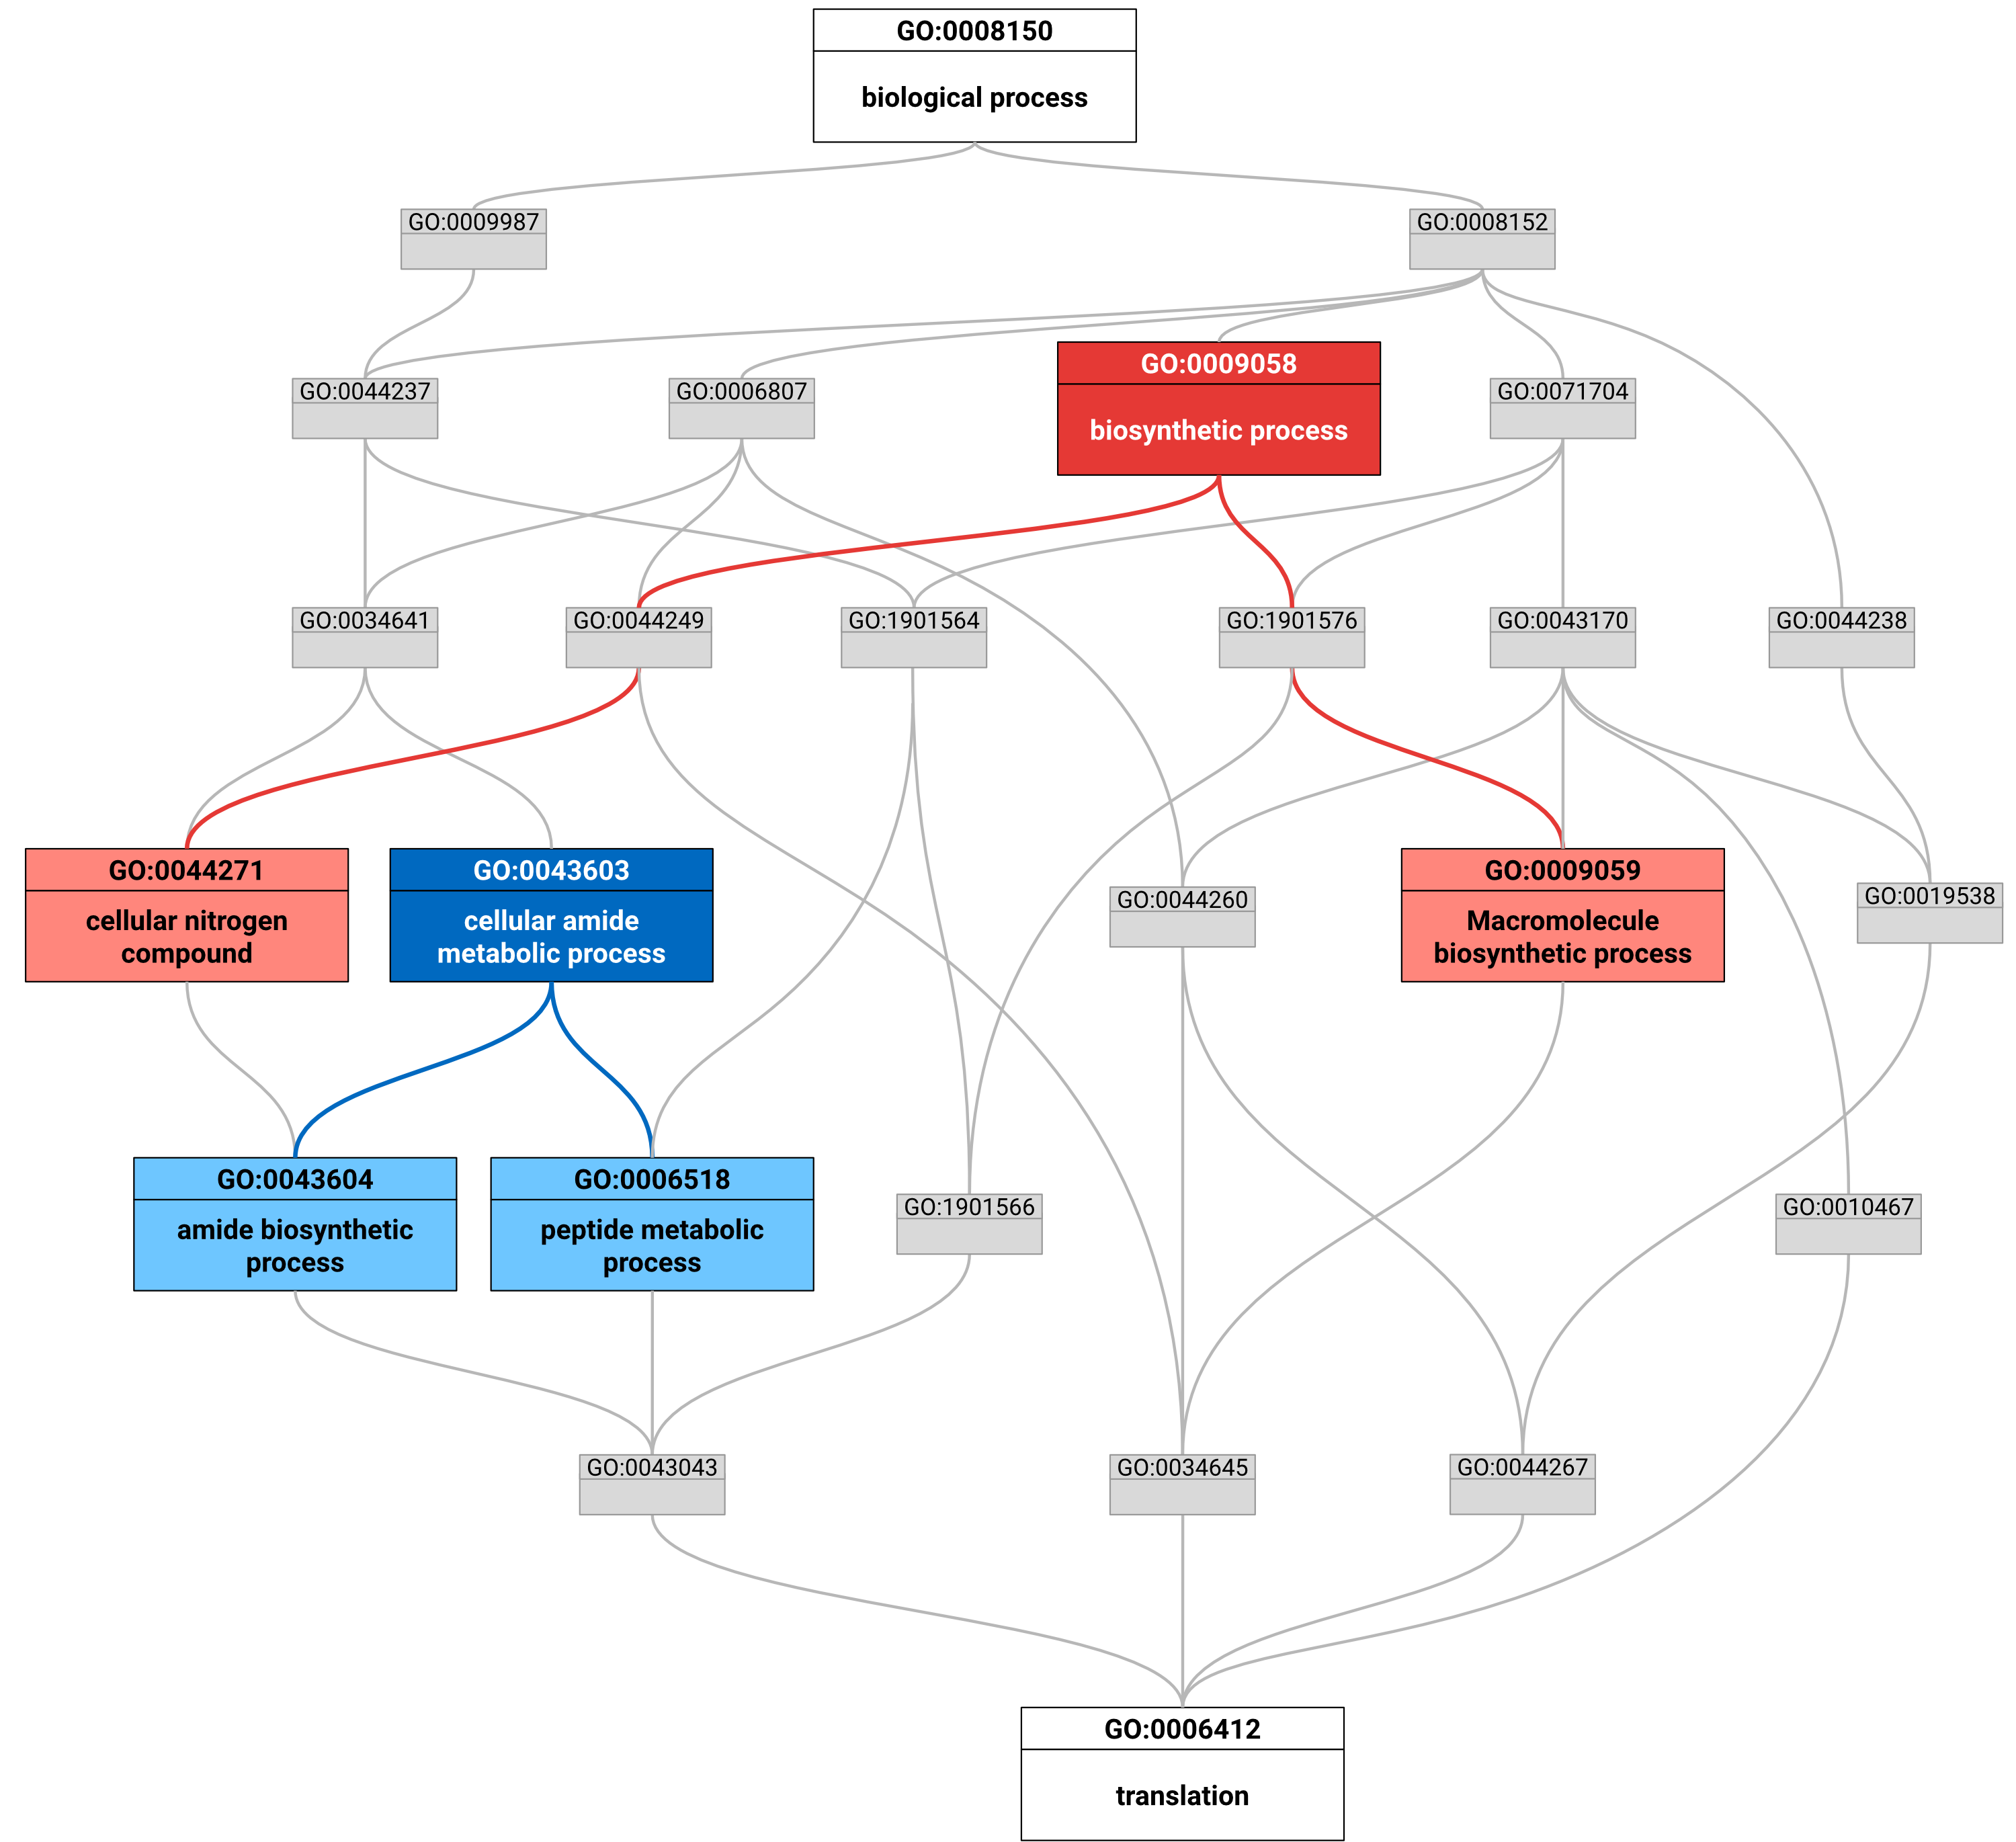
\includegraphics{resources/figures/chapter4_megago_biological_process_excerpt.png}
\caption{Excerpt of the biological process domain of the Gene Ontology
showing all parent terms up to the root for ``translation''
(GO:0006412). The root GO term ``biological process`` (GO:0008150) has
multiple children. The most specific term ``translation'', in contrast,
has multiple parents. When comparing the two terms GO:0044267 and
GO:0034645 (portrayed in light red), we find two different lowest common
ancestors: GO:0044249 and GO:1901576 (dark red). Only one of these,
however, can be the most informative common ancestor (MICA), that is,
the common ancestor with the highest information content for the terms
in light red. Because an IC of 1.52 is larger than 1.48, the GO:0044249
is the MICA. The terms GO:0043604 and GO:0006518 (in light blue) are
more similar than the two terms we previously described and have only
one lowest common ancestor, which is also automatically the MICA for
these terms: GO:0043603 (in dark blue). IC, information content; *, most
informative common
ancestor.\label{fig:megago_biological_process_excerpt}}
\end{figure}

Whereas this highly branched graph structure of GO allows flexible
annotation at various levels of detail, it also creates problems when
the results from one data set are compared to those of another data set.
Indeed, even though two terms may be closely linked in the GO tree and
are therefore highly similar (e.g., as parent and child terms or as
sibling terms), the typically employed exact term matching will treat
these terms as wholly unrelated, as the actual GO terms (and their
accession numbers) are not identical. This problem is illustrated in a
study by (Sajulga \emph{et al.}, 2020), where a multisample data set was
analyzed using several metaproteomics tools. The resulting GO terms were
then compared using exact matching. The overlap between the result sets
was quantified using the Jaccard index and was found to be low. As
previously explained, this low similarity is likely the result of the
limitations of the exact term matching approach.

There is thus a clear need for a more sophisticated GO term comparison
that takes into account the existing relationships in the full GO tree.
However, most existing tools that provide such comparison are based on
enrichment analyses (Huang \emph{et al.}, 2009; Waardenberg \emph{et
al.}, 2015; Fruzangohar \emph{et al.}, 2013). In such analyses, a list
of genes is mapped to GO terms, which are then analyzed for enriched
biological phenomena. As a result, to the best of our knowledge, no
tools allow the direct comparison of large functional data sets against
each other, nor are these able to provide metrics to determine how
functionally similar data sets are.

We therefore present MegaGO, a tool for comparing the functional
similarity between large sets of GO terms. MegaGO calculates a pairwise
similarity score between multiple sets of GO terms for each of the three
GO domains and can do so in seconds, even on platforms with limited
computational capabilities.

\hypertarget{implementation-1}{%
\section{Implementation}\label{implementation-1}}

To measure the similarity between sets of GO terms, we first need to
measure the similarity of two individual terms. We compare two terms
using the Lin semantic similarity metric, which can take on a value
between 0 and 1 (Supplementary Formula 1a). The Lin semantic similarity
is based on the ratio of the information content of the most informative
common ancestor (MICA) to the average of the terms' individual
information content.

The information content (Supplementary Formula 1b) is computed by
estimating the terms' probability of occurrence (Supplementary Formula
1c), including that of all of their children. Term frequencies are
estimated based on the manually curated SwissProt database (The UniProt
Consortium, 2019). As a result, a high-level GO term such as
``biological process'' (through its many direct or indirect child terms)
will be present in all data sets and thus carries little information. A
more specific term such as ``translation'' (or any of its potential
child terms) will occur less frequently and thus will be more
informative (\autoref{fig:megago_biological_process_excerpt}). To
finally calculate the similarity of two terms, we compare their
information content with that of their shared ancestor that has the
highest information content, the MICA. If the information content of the
MICA is similar to the terms' individual information content, then the
terms are deemed to be similar. The dissimilar terms ``peptide
biosynthetic process'' and ``cellular macromolecule biosynthetic'' are
situated further from their MICA ``cellular biosynthetic process'' than
the similar terms ``amide biosynthetic process'' and ``peptide metabolic
process'' with their respective MICA ``cellular amide metabolic
process'' (\autoref{fig:megago_biological_process_excerpt}).

MegaGO, however, can compare not only two terms but also sets of GO
terms. More specifically, two sets of GO terms can be compared via the
web application, but an unlimited number of sets can be compared via the
command line tool. Note that in these sets, duplicate GO terms will be
removed so that each GO term will be equally important, regardless of
how often it is provided by the user. To compare the sets of GO terms,
pairwise term similarities are aggregated using the Best Matching
Average (BMA, Supplementary Formula 2) (Schlicker \emph{et al.}, 2006).
For each GO term in the first input data set, the BMA finds the GO term
with the highest Lin semantic similarity in the second data set and
averages the values of these best matches. Moreover, MegaGO calculates
the similarity for each of the three domains of the gene ontology
(molecular function, biological process, and cellular component), as GO
terms from distinct domains do not share parent terms. The general
overview of MegaGO is shown in \autoref{fig:megago_workflow_overview}.

\begin{figure}
\centering
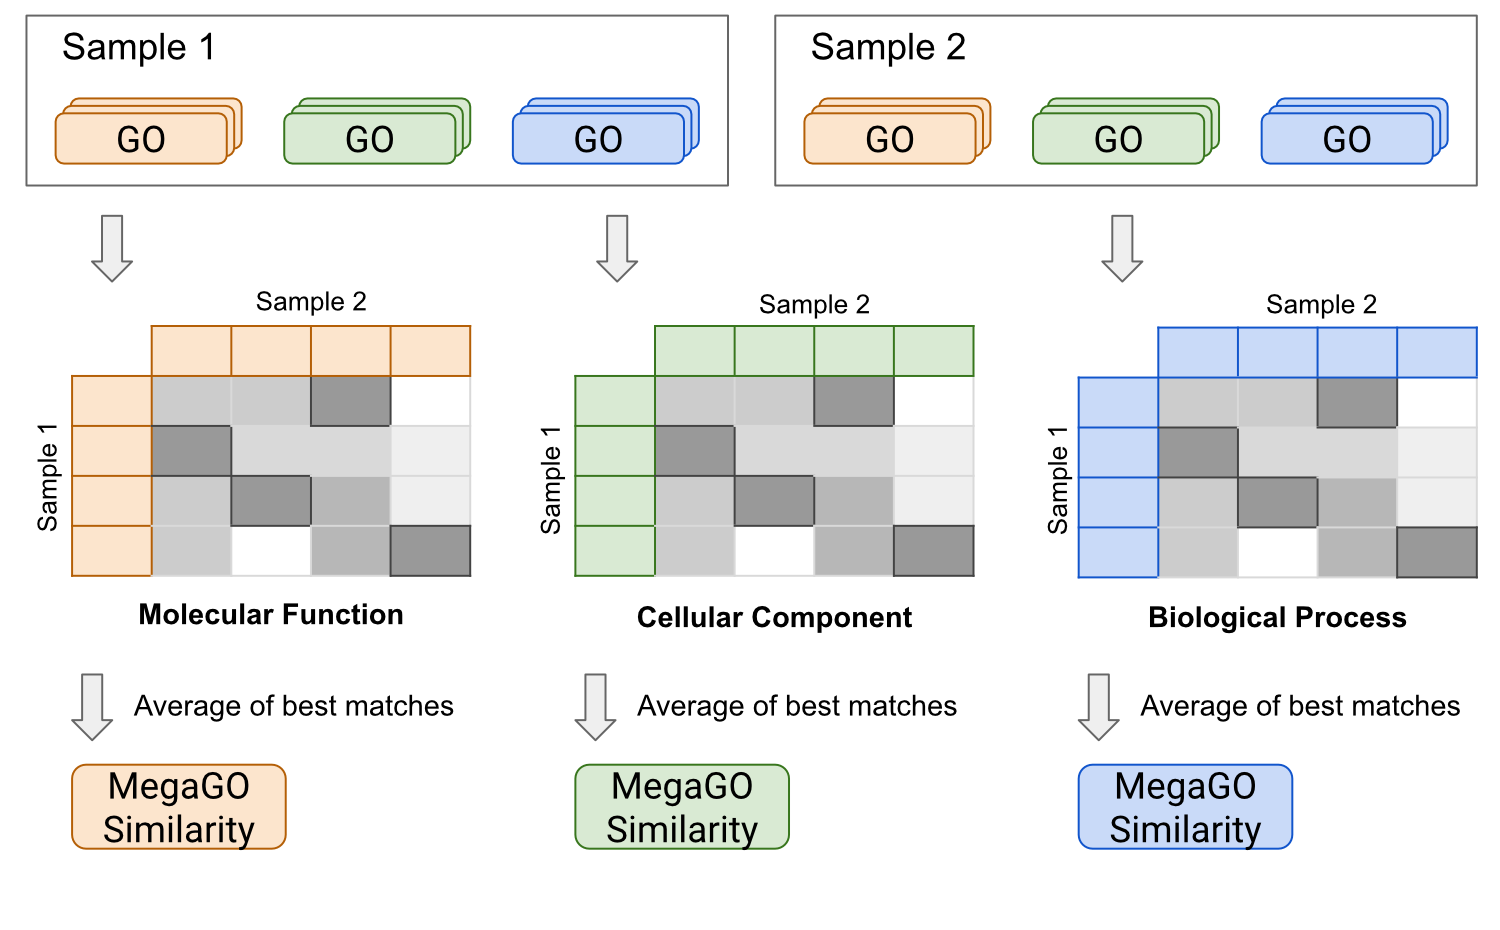
\includegraphics{resources/figures/chapter4_megago_workflow_overview.png}
\caption{Overview of MegaGO workflow. The Gene Ontology (GO) terms of
each sample set are separated into three GO domains: molecular function,
cellular component, and biological process. Each term of each sample set
is compared to every term in the other set that is from the same domain.
The match with highest similarity for each term is then selected, and
the average across all of these best matches is
calculated.\label{fig:megago_workflow_overview}}
\end{figure}

MegaGO is implemented in Python, is installable as a Python package from
PyPi, and can easily be invoked from the command line. The GOATOOLS
(Klopfenstein \emph{et al.}, 2018) library is used to read and process
the Gene Ontology and to compute the most informative common ancestor of
two GO terms, which are both required to compute the information content
value (Supplementary Formula 1, p(go)). GO term counts are recomputed
with every update of SwissProt, and a new release is automatically
published bimonthly to PyPi, which includes the new data set. Automated
testing via GitHub Actions is in place to ensure correctness and
reproducibility of the code. In addition, we also developed a
user-friendly and easily accessible web application that is available on
https://megago.ugent.be. The backend of the web application is developed
with the Flask web framework for Python, and the frontend uses Vue. Our
web application has been tested on Chromium-based browsers (Chrome,
Edge, and Opera) as well as Mozilla Firefox and Safari. The MegaGO
application is also available as a Docker-container on Docker Hub
(https://hub.docker.com/repository/docker/pverscha/mega-go) and can be
started with a single click and without additional configuration
requirements. Our Docker container is automatically updated at every
change to the underlying MegaGO code. All code is freely available under
the permissive open source MIT license on https://github.com/MEGA-GO/.
Documentation for our Python script can be found on our Web site:
https://megago.ugent.be/help/cli. A guide on how to use the web
application is also available: https://megago.ugent.be/help/web.

MegaGO is cross-platform and runs on Windows, macOS, and Linux systems.
The system requirements are at least 4 GiB of memory and support for
either Python 3.6 (or above) or the Docker runtime.

\hypertarget{validation}{%
\section{Validation}\label{validation}}

To validate MegaGO, we reprocessed the functional data from (Easterly
\emph{et al.}, 2019). This data set consists of 12 paired oral
microbiome samples that were cultivated in bioreactors. Each sample was
treated with and without sucrose pulsing, hereafter named ws and ns
samples, respectively. Each sample contains mass-spectrometry-based
proteomics measurements, and all samples were annotated with 1718 GO
terms on average. We calculated the pairwise similarity for each of the
300 sample combinations, which took less than 1 min for a single sample
pair on the web version of MegaGO. This resulted in a MegaGO similarity
score for each of the three GO domains for each sample combination.
These similarities were then hierarchically clustered and visualized in
a heatmap. All data and intermediate steps of our data analysis are
available at https://github.com/MEGA-GO/manuscript-data-analysis/ and
can be reproduced with the command line tool using the --heatmap option.

In the heatmap (\autoref{fig:megago_heatmap}), we can observe that the
two sample groups cluster together, except for 730ns and 733ns that are
clustered in the ws sample group. These two samples were also identified
as outliers in (Easterly \emph{et al.}, 2019) and 733ns was originally
also identified as both a taxonomic and functional outlier in (Rudney
\emph{et al.}, 2015). Similar results can be observed for the GO domain
``molecular function'' (Supplementary Figure 1). The MegaGO
similarity-based clustering of ``cellular component'' GO terms
(Supplementary Figure 2) has two additional samples clustered outside of
their treatment group: 852ws in the ns cluster and 861ns in the ws
group. Again, these patterns can also be found in previous analyses:
852ws is placed in direct proximity of the ns samples in the principal
component analysis (PCA) of the HOMINGS analysis by Rudney et al., and
861ns is closest to 730ns and 733ns in PCA of Rudney et al.'s taxonomic
analysis. Interestingly, subjects 730 and 852 were the only ones without
active carious lesions, which could cause their divergence in the
similarity analyses.

\begin{figure}
\centering
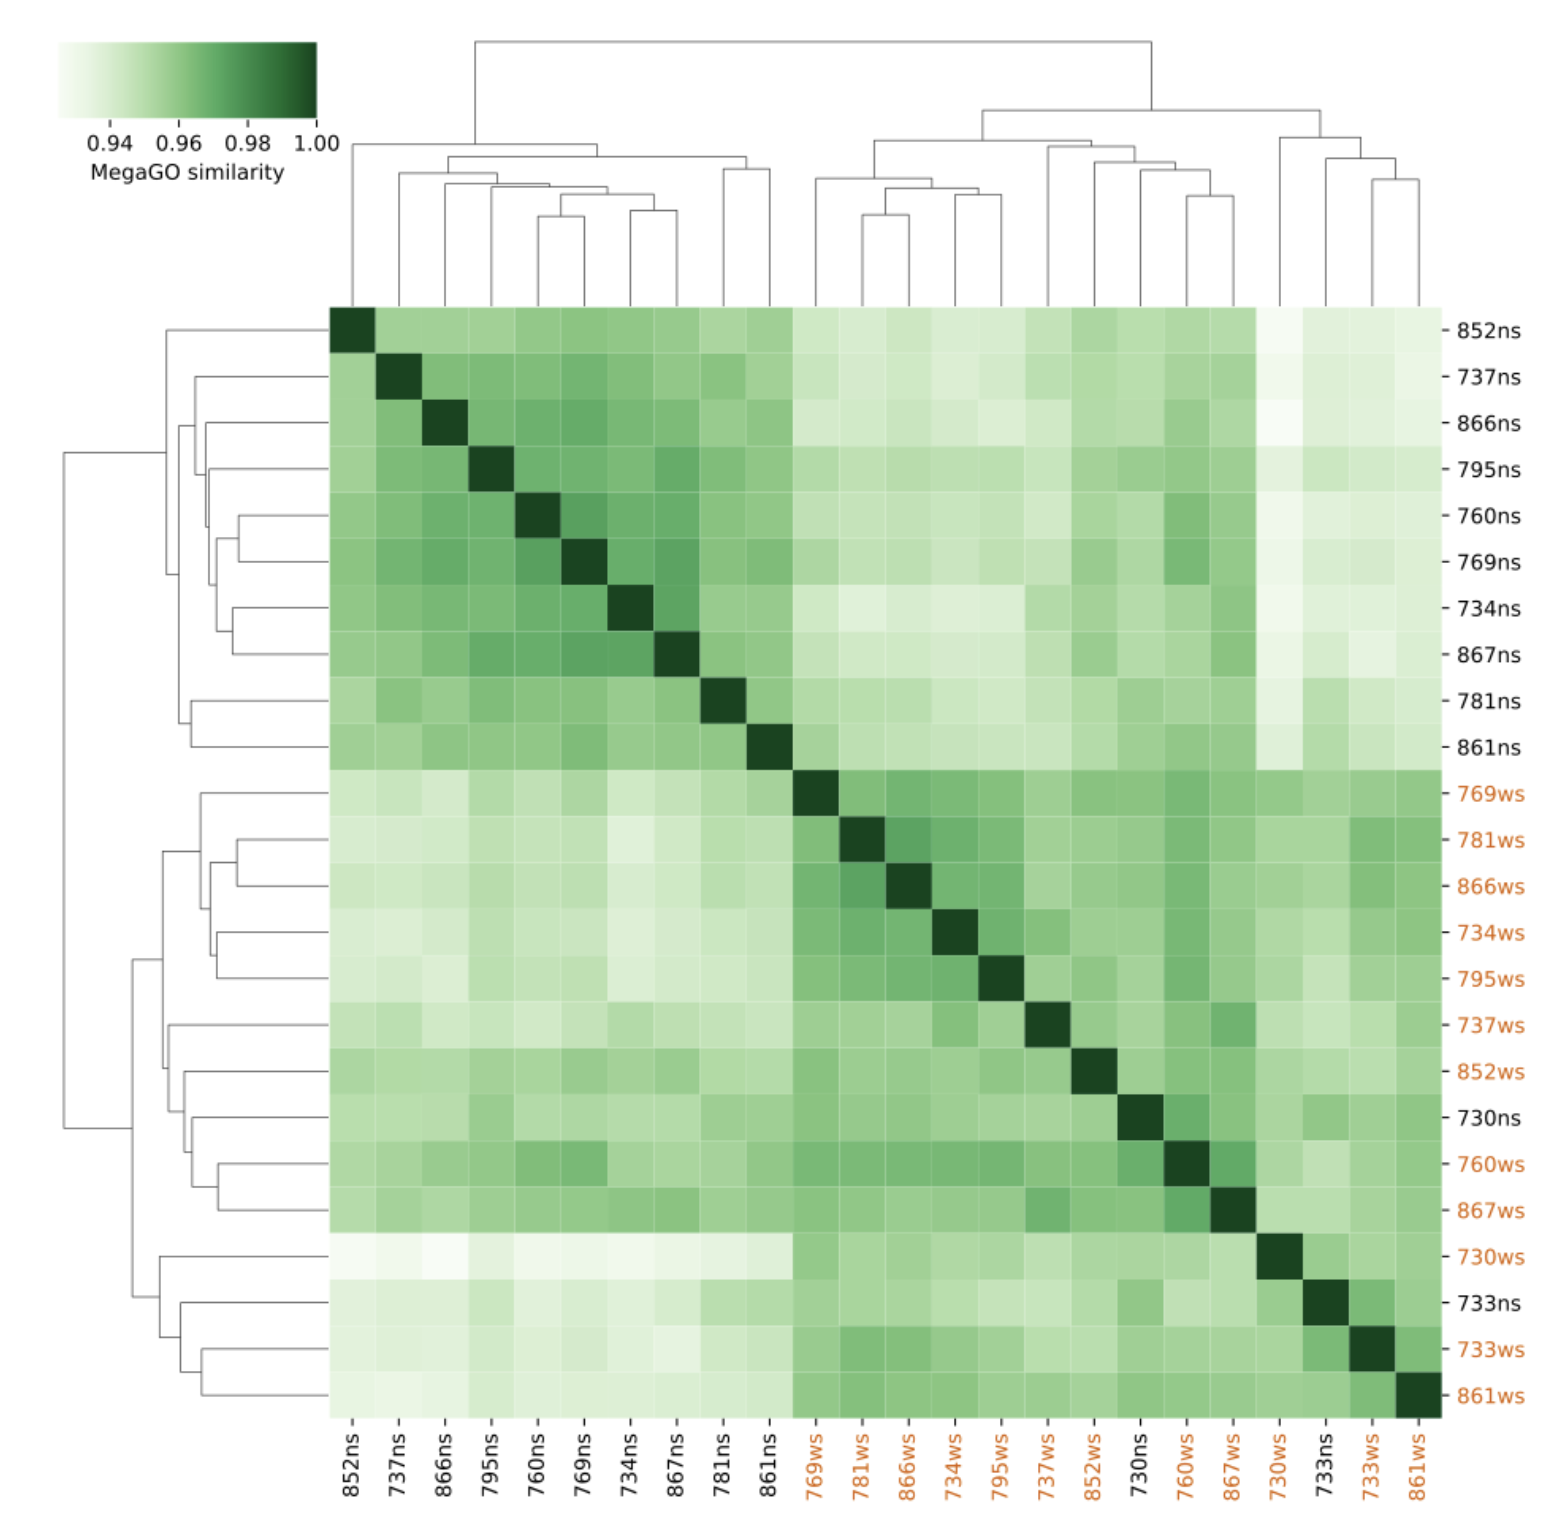
\includegraphics{resources/figures/chapter4_megago_heatmap_example.png}
\caption{Hierarchically clustered heatmap comparing MegaGO similarities
for the GO domain ``biological process'' for each of the samples from
(Easterly \emph{et al.}, 2019) Samples that are treated with sucrose
pulsing are labeled as ``ws'' and are displayed in
orange.\label{fig:megago_heatmap}}
\end{figure}

Results produced by MegaGO are thus in close agreement with prior
analyses of the same data, showing that MegaGO offers a valid and very
fast approach for comparing the functional composition of samples.

\hypertarget{conclusions}{%
\section{Conclusions}\label{conclusions}}

MegaGO enables the comparison of large sets of GO terms, allowing users
to efficiently evaluate multiomics data sets containing thousands of
terms. MegaGO separately calculates a similarity for each of the three
GO domains (biological process, molecular function, and cellular
component). In the current version of MegaGO, quantitative data are not
taken into account, thus giving each GO term identical importance in the
data set.

MegaGO is compatible with any upstream tool that can provide GO term
lists for a data set. Moreover, MegaGO allows the comparison of
functional annotations derived from DNA-, RNA-, and protein-based
methods as well as combinations thereof.

\hypertarget{acknowledgements-2}{%
\section{Acknowledgements}\label{acknowledgements-2}}

We acknowledge the European Bioinformatics Community for Mass
Spectrometry (EuBIC-MS). This project found its origin at the EuBIC
Developers' 2020 meeting (Ashwood \emph{et al.}, 2020) in Nyborg,
Denmark. We thank Thilo Muth (Bundesanstalt für Materialforschung und
-prüfung, Berlin, Germany) and Stephan Fuchs (Robert Koch Institute,
Berlin, Germany) for their support. P.V., T.V.D.B., L.M., and B.M.
acknowledge the Research Foundation - Flanders (FWO) (grants 1164420N,
1S90918N, G042518N, and 12I5220N). L.M. also acknowledges support from
the European Union's Horizon 2020 Programme under grant agreement 823839
(H2020-INFRAIA-2018-1). H.S. and B.Y.R. acknowledge support by Deutsche
Forschungsgemeinschaft (DFG; grant numbers RE3474/5-1 and RE3474/2-2)
and the BMBF-funded de.NBI Cloud within the German Network for
Bioinformatics Infrastructure (de.NBI; 031A537B, 031A533A, 031A538A,
031A533B, 031A535A, 031A537C, 031A534A, and 031A532B).

\hypertarget{unipept-cli-2.0-adding-support-for-visualisations-and-functional-annotations}{%
\chapter{Unipept CLI 2.0: adding support for visualisations and
functional
annotations}\label{unipept-cli-2.0-adding-support-for-visualisations-and-functional-annotations}}

\textbf{Abstract} Unipept (Mesuere \emph{et al.}, 2012) is a collection
of tools developed for fast metaproteomics data analysis. The Unipept
ecosystem consists of a web application, an application programming
interface (API) as a web service (Mesuere \emph{et al.}, 2016) and a
command-line interface (CLI) (Mesuere \emph{et al.}, 2018). The key
strengths of Unipept are its speed, its ease-of-use and the extensive
use of interactive data visualization in the analysis results. The
Unipept database is derived from the UniProt (UniProt, 2019) KB and
consists of tryptic peptides linked with taxonomic and functional
annotations. Unipept initially launched with support for taxonomic
analysis of metaproteomics data in 2012. Version 4.0 (Gurdeep Singh
\emph{et al.}, 2019) of the Unipept web application was launched in
November 2018 and extended the web interface with support for functional
annotations such as Gene Ontology (GO) terms (Ashburner \emph{et al.},
2000), Enzyme Commission (EC) numbers (Webb, 1992) and InterPro entries
(Hunter \emph{et al.}, 2009).

\hypertarget{introduction-3}{%
\section{Introduction}\label{introduction-3}}

Unipept (Mesuere \emph{et al.}, 2012) is a collection of tools developed
for fast metaproteomics data analysis. The Unipept ecosystem consists of
a web application, an application programming interface (API) as a web
service (Mesuere \emph{et al.}, 2016) and a command-line interface (CLI)
(Mesuere \emph{et al.}, 2018). The key strengths of Unipept are its
speed, its ease-of-use and the extensive use of interactive data
visualization in the analysis results. The Unipept database is derived
from the UniProt (The UniProt Consortium, 2019) KB and consists of
tryptic peptides linked with taxonomic and functional annotations.
Unipept initially launched with support for taxonomic analysis of
metaproteomics data in 2012. Version 4.0 (Gurdeep Singh \emph{et al.},
2019) of the Unipept web application was launched in November 2018 and
extended the web interface with support for functional annotations such
as Gene Ontology (GO) terms (Ashburner \emph{et al.}, 2000), Enzyme
Commission (EC) numbers (Webb, 1992) and InterPro entries (Hunter
\emph{et al.}, 2009).

The GO terms are organized into three different domains: `cellular
components', `molecular functions' and `biological processes'. Every
GO-term is associated with exactly one domain and consists of a name, an
identifier and an exact definition. The EC numbers can be used to
classify enzymes, based on the chemical reactions that they catalyze.
Every EC number consists of four numbers, separated by a dot, yielding a
hierarchical classification system with progressively finer enzyme
classifications. InterPro is a database that consists of predictive
models collected from external databases that can be classified into
five different categories. More information about functional annotation
in metaproteomics can be found in the study by (Schiebenhoefer \emph{et
al.}, 2019).

For each input peptide, Unipept finds all functional annotations
associated with all of the UniProt entries in which the peptide occurs.
All found functions are listed in order of decreasing number of peptides
associated with this function.

In this article, we present several new additions to the Unipept API and
CLI which allow third-party applications {[}such as Galaxy-P (Jagtap
\emph{et al.}, 2015){]} to integrate the new functional analysis
capabilities provided by Unipept.

\hypertarget{materials-and-methods}{%
\section{Materials and methods}\label{materials-and-methods}}

The Unipept API is a high-performance web service that responds in a
textual format (JSON) to HTTP-requests from other applications or tools
and allows to integrate the services provided by Unipept into other
workflows. Unipept's CLI is a Ruby-based application and high-level
entry point which allows users to actively query Unipept's database.
Compared to the API, users do not need to compile API-requests manually
but can rely on the CLI to automatically do so in a parallelized way. In
addition, it supports multiple input and output formats such as FASTA
and CSV.

The Unipept database and web application were recently expanded to
include GO terms, EC numbers and InterPro entries. These new annotations
are now also available from newly developed API-endpoints and
CLI-functions, providing structured access to this functional
information.

Most of the newly developed endpoints support batch retrieval of
information for a list of peptides. In this case, the API returns a list
of objects where each object in the response corresponds with
information associated with one of the input peptides. Every
API-endpoint is accompanied by an identically named CLI-function, which
provides the user with the ability to import data from or export data to
various specifically formatted files. In addition, version 2 of the
Unipept CLI introduces the ability to produce interactive visualizations
directly from the command line.

Among other information, the Unipept tryptic peptide analysis lists
functional annotations associated with a given tryptic peptide. These
data are aggregated because a peptide can occur in multiple proteins
that each can have multiple functional annotations. For each annotation,
we also return the amount of underlying proteins that match with this
specific annotation.

Some applications require all known information for a list of tryptic
peptides. The `pept2funct' function is a combination of the preceding
three endpoints and returns all functional annotations associated with
the given tryptic peptide. `peptinfo' on the other hand, returns all the
available information for one or more tryptic peptides. All functional
annotations for this peptide are part of the response, as well as the
lowest common ancestor for this peptide. Both functions also support
splitting the GO terms and InterPro entries over the respective domains,
and naming information can optionally be retrieved.

The `taxa2tree' function constructs a tree from a list of NCBI taxon
ids. This tree is an aggregation of the lineages that correspond with
the given taxa and can be exported as three distinct output formats:
JSON, HTML and as a URL. The HTML and URL representation of a taxonomic
tree both provide three interactive data visualizations, albeit with
different possibilities. A generated HTML-string first needs to be
stored in a file before it can be rendered by a browser and cannot be
easily shared with other people but is easily editable. A URL on the
other hand is simply a shareable link to an online service that hosts
all interactive visualizations.

\hypertarget{conclusion-1}{%
\section{Conclusion}\label{conclusion-1}}

Version 2.0 of the Unipept API and CLI is a significant update that
provides fast and easy access to the powerful analysis pipeline of
Unipept. In addition to the existing taxonomic analysis, it now features
multiple functional annotations which will enable users to gain new
insights into complex ecosystems. These new features can easily be
integrated into third-party tools such as the MetaProteome Analyzer
(Muth \emph{et al.}, 2018). Galaxy-P, a highly used workflow integration
system, is already successfully making use of the novel analysis
functions that are introduced with this new release.

\hypertarget{funding}{%
\section{Funding}\label{funding}}

This work was supported by the Research Foundation---Flanders (FWO)
{[}1164420N to P.V.; 12I5220N to B.M.; 1S90918N to T.V.D.B.; G042518N to
L.M.; 12S9418N to C.D.T.{]}.

\hypertarget{unipept-visualizations-an-interactive-visualization-library-for-biological-data}{%
\chapter{Unipept Visualizations: an interactive visualization library
for biological
data}\label{unipept-visualizations-an-interactive-visualization-library-for-biological-data}}

\markright{\textsf{Novel visualizations tailored at biological data}}

\textbf{Abstract} The Unipept Visualizations library is a JavaScript
package to generate interactive visualizations of both hierarchical and
non-hierarchical quantitative data. It provides four different
visualizations: a sunburst, a treemap, a treeview and a heatmap. Every
visualization is fully configurable, supports TypeScript and uses the
excellent D3.js library. The Unipept Visualizations library is available
for download on NPM: \url{https://npmjs.com/unipept-visualizations}. All
source code is freely available from GitHub under the MIT license:
\url{https://github.com/unipept/unipept-visualizations}.

\hypertarget{introduction-4}{%
\section{Introduction}\label{introduction-4}}

Unipept is an ecosystem of software tools for the analysis of
metaproteomics datasets that consists of a web application (Gurdeep
Singh \emph{et al.}, 2019), a desktop application (Verschaffelt \emph{et
al.}, 2021), a command line interface (Verschaffelt \emph{et al.}, 2020)
and an application programming interface. It provides taxonomic and
functional analysis pipelines for metaproteomics data and highly
interactive data visualizations that help interpret the outcome of these
analyses.

We developed custom visualizations used for Unipept from scratch because
existing libraries, such as Krona (Ondov \emph{et al.}, 2011), were
lacking essential features or were hard to integrate. They were designed
as generic tools to visualize hierarchical quantitative data and can
therefore also be used to visualize data from nonproteomics origins. To
facilitate reuse of these broadly usable components, we have isolated
the visualizations from the main Unipept project and made them available
as a standalone package that can easily be reused by other software
tools. We released this package under the permissive MIT open-source
license, so researchers from other disciplines are free to reuse these
visualizations and connect them to their own data sources. Currently,
our visualizations are already incorporated in TRAPID 2.0, a web
application for the analysis of transcriptomes ((Bucchini \emph{et al.},
2021) and UMGAP, the Unipept MetaGenomics Pipeline (Van der Jeugt
\emph{et al.}, 2022).

\hypertarget{visualizations}{%
\section{Visualizations}\label{visualizations}}

We currently provide four highly interactive data visualizations that
are all designed for a specific purpose: a sunburst, a treeview, a
treemap and a heatmap. The sunburst
(\autoref{fig:visualizations_overview}a), treeview
(\autoref{fig:visualizations_overview}d) and treemap
(\autoref{fig:visualizations_overview}b) can be used to visualize
quantitative hierarchical data and are designed to depict the
parent--child relationship of a hierarchy of nodes as clearly as
possible, while still incorporating the strength of the relationship
between, or the counts associated with, connected nodes. The heatmap
(\autoref{fig:visualizations_overview}c), conversely, is not suitable to
visualize hierarchical information but displays a magnitude in two
dimensions, including optional clustering and dendrogram rendering.

\begin{figure}
\centering
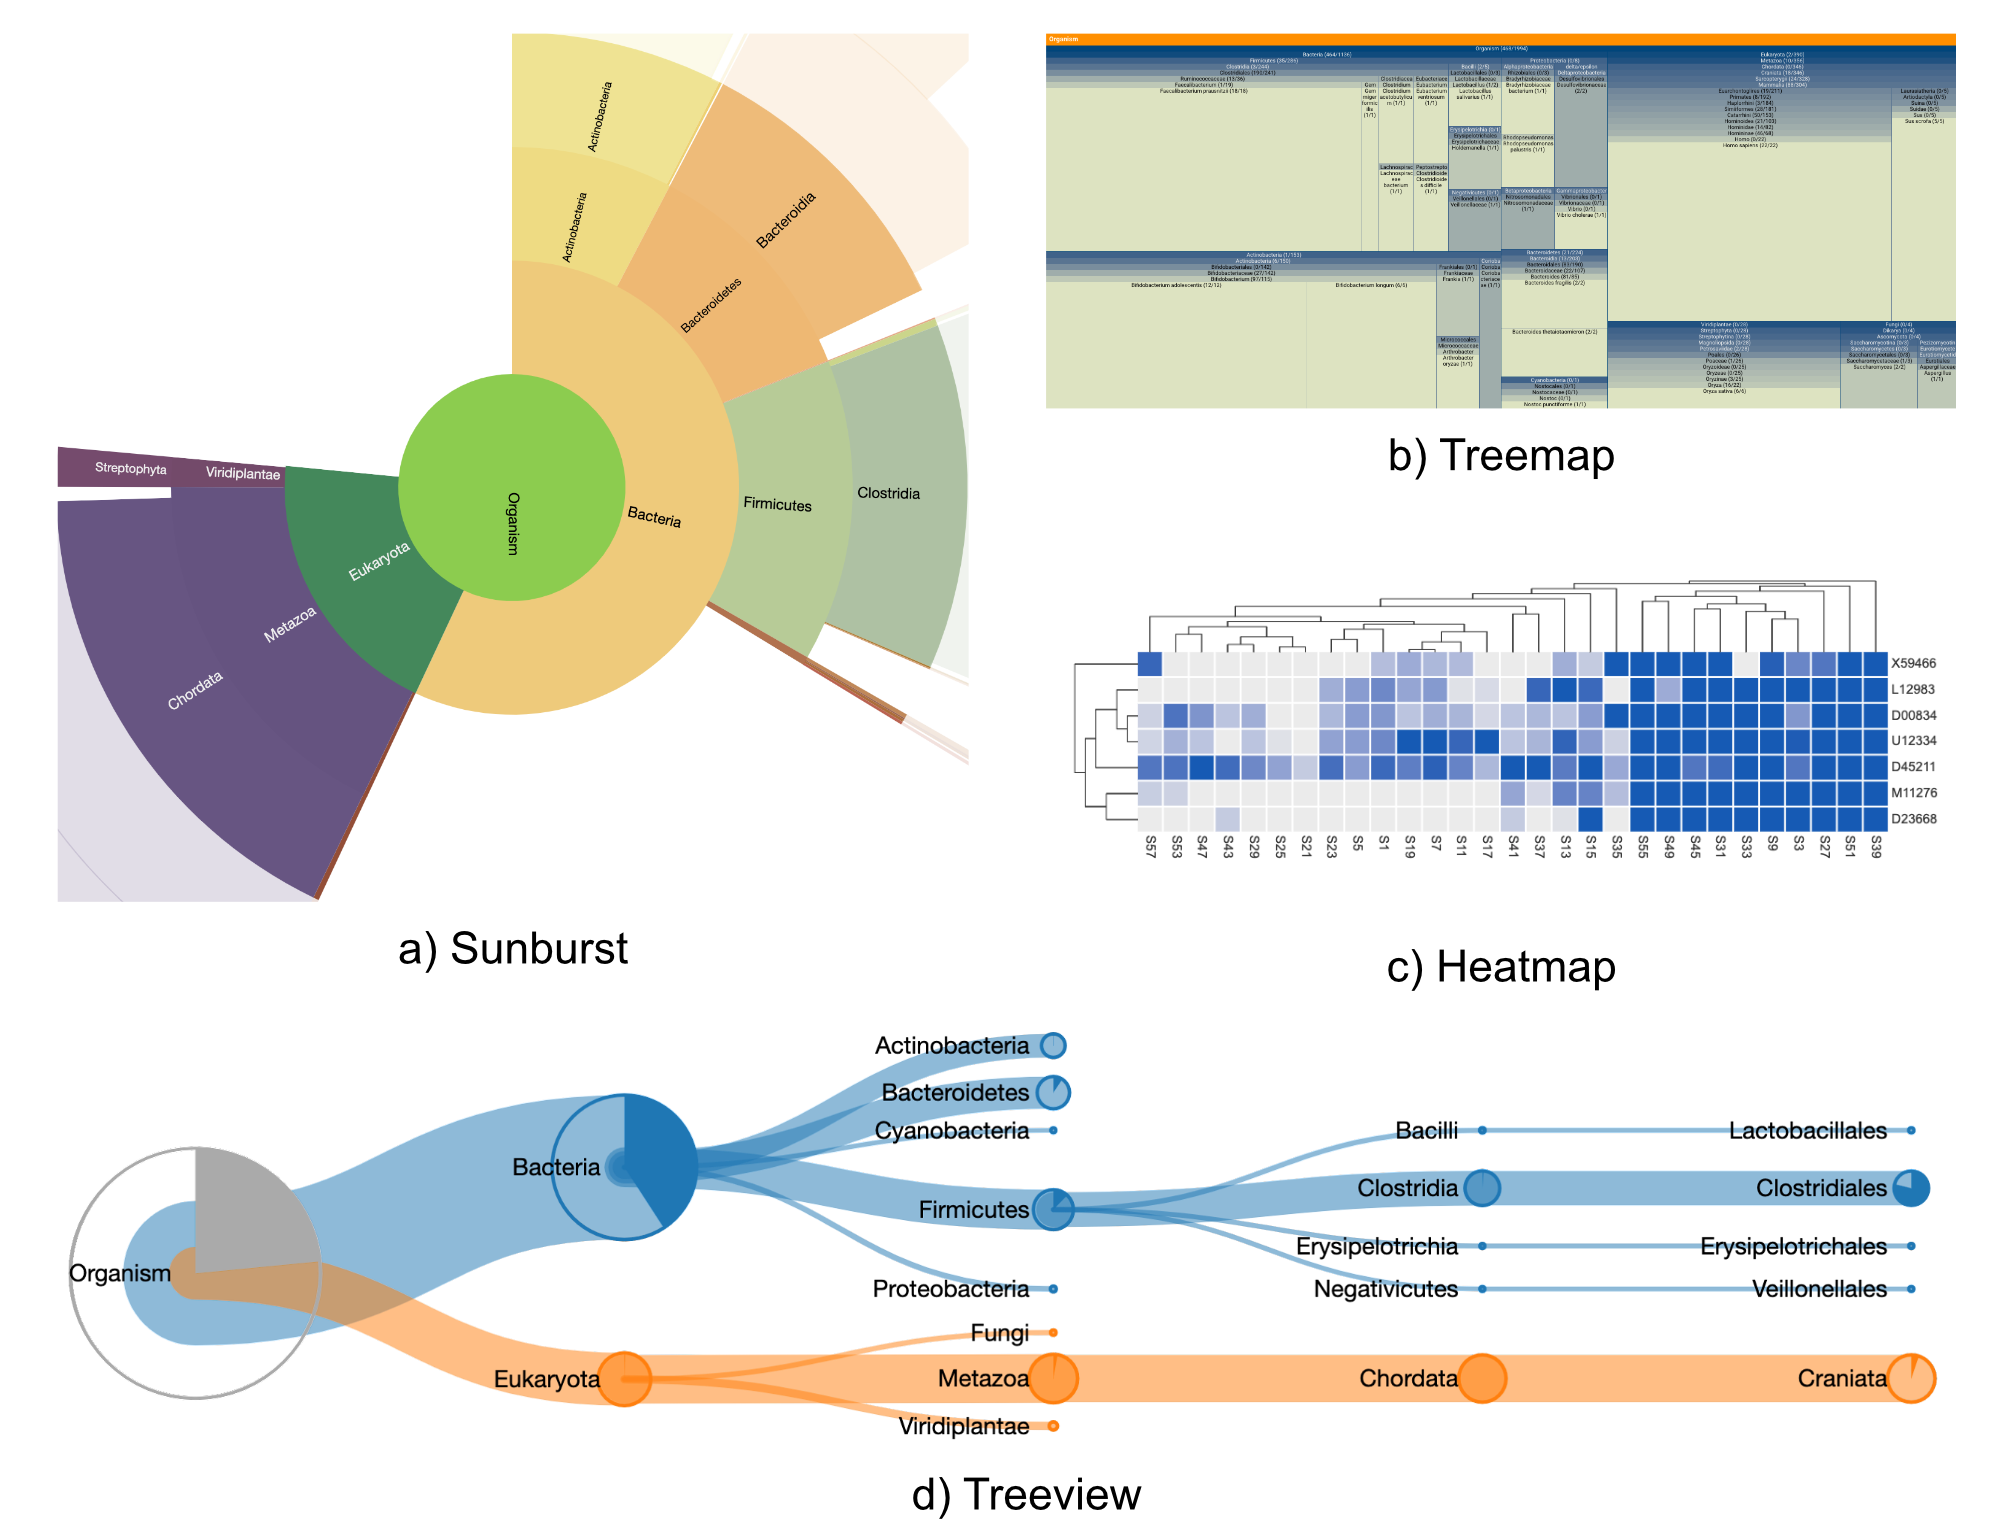
\includegraphics{resources/figures/chapter6_visualizations_overview.png}
\caption{Overview of the visualizations currently provided by the
Unipept Visualizations library. All examples were generated with default
configuration settings, except for the heatmap for which the setting
`dendrogramEnabled' was set to
`true'.\label{fig:visualizations_overview}}
\end{figure}

\hypertarget{quantitative-hierarchical-data-visualizations}{%
\subsection{Quantitative hierarchical data
visualizations}\label{quantitative-hierarchical-data-visualizations}}

Hierarchical data occurs throughout a variety of bioinformatics
disciplines. In the metaproteomics research area alone, many examples of
hierarchical data exist, such as the hierarchical structure of the NCBI
taxonomy (Schoch \emph{et al.}, 2020), the hierarchy imposed by the
enzyme commission numbers and the gene ontology terms
(The~Gene~Ontology~Consortium, 2019). In most cases, quantitative data
are available for multiple nodes at many levels in the hierarchy. For
example, Unipept assigns peptide counts to taxa that are scattered
around the NCBI taxonomy, including identifications that are highly
specific (near leaves of the tree) or lack deep taxonomic resolution
(near the root of the tree). Being able to interactively zoom in and out
on the hierarchical data enables exploratory analysis.

The three visualizations for hierarchical data provided by our package
take input data in the same hierarchical format, making it trivial to
switch between the different types of visualization once the input data
are formatted correctly.

\hypertarget{quantitative-non-hierarchical-data-visualizations}{%
\subsection{Quantitative non-hierarchical data
visualizations}\label{quantitative-non-hierarchical-data-visualizations}}

A heatmap (\autoref{fig:visualizations_overview}c) is a well-known
visualization that consists of a two-dimensional grid of cells in which
each cell is assigned a specific color from a scale corresponding to its
magnitude. The heatmap implementation in our package provides this
functionality in an extensively customizable form. Users can reorganize
elements, change the color scheme and update label information, among
other operations. All values are also automatically normalized to a
{[}0, 1{]}-interval.

As neighboring rows and columns in the input data can have very distinct
values, and as this can interfere with reasoning about the heatmap, it
is important to group similar values. Our implementation achieves this
through hierarchical clustering based on the UPGMA algorithm (Sokal and
Michener, 1958). The produced grouping of rows and columns is further
clarified by an optional dendrogram that can be plotted alongside each
axis of the heatmap.

However, after clustering, it can still occur that two consecutive
leaves in a dendrogram are quite dissimilar due to the \(2^n−1\)
possible linear orderings that can be derived from a dendrogram (a
dendrogram contains \(n - 1\) flipping points for which both children
can be switched). This can be addressed by reordering the leaves of the
tree, as the orientation of the children of all n nodes in a dendrogram
can be flipped without affecting the integrity of the dendrogram itself.
Our heatmap implementation uses the Modular Leaf Ordering technique
(Sakai \emph{et al.}, 2014) to reorder all leaves of the dendrogram such
that the distance between consecutive leaves is minimized. This
technique is a heuristic that performs very well in comparison to the
more resource-intensive Optimal Leaf Ordering (Bar-Joseph \emph{et al.},
2001) or Gruvaeus--Wainer algorithms (Gruvaeus and Wainer, 1972).

\hypertarget{implementation-2}{%
\section{Implementation}\label{implementation-2}}

The visualization package has been developed with D3 (Bostock \emph{et
al.}, 2011) and TypeScript (Bierman \emph{et al.}, 2014) and every
visualization is displayed in the web browser with one of two
technologies: SVG or HTML5 canvas. SVG's are easy-to-use and are
scalable by nature but often lack necessary performance for complex
interactive visualizations. HTML5 canvas, in contrast, provides much
better performance using a rasterized image.

Every visualization is presented as a single JavaScript class and
provides a full set of configuration options to extend and configure the
visualization. New versions of the package will automatically be
published on NPM (\url{https://npmjs.org}) and GitHub
(\url{https://github.com/unipept/unipept-visualizations}), so that any
project depending on it package can always use the latest version.

We also provide an extensive set of documentation resources that ease
the adoption process of our package, as well as a collection of live
notebooks (see
\url{https://observablehq.com/collection/@unipept/unipept-visualizations}).
These notebooks provide interactive and editable examples that
demonstrate the full potential and guide users through the different
configuration options. The code and resources that make up the live
notebooks can be modified online and provide a very convenient way to
try out the package.

\hypertarget{funding-1}{%
\section{Funding}\label{funding-1}}

This work has been supported by the Research Foundation---Flanders (FWO)
{[}1164420N to P.V.; 12I5220N to B.M.; G042518N to L.M.{]}.

\hypertarget{other-projects-1}{%
\chapter{Other projects}\label{other-projects-1}}

\markright{\textsf{Other projects conducted during my PhD}}

During the course of my career as a PhD student, I have also been
working on a lot of different research projects for which I was not the
main contributor, but for which I, nonetheless, provided a significant
addition. I have selected two of these projects and included them as
sections in this chapter.

\hypertarget{pout2prot-an-efficient-tool-to-create-protein-subgroups-from-percolator-output-files}{%
\section{Pout2Prot: An efficient tool to create protein (sub)groups from
Percolator output
files}\label{pout2prot-an-efficient-tool-to-create-protein-subgroups-from-percolator-output-files}}

\textbf{Abstract} In metaproteomics, the study of the collective
proteome of microbial communities, the protein inference problem is more
challenging than in single-species proteomics. Indeed, a peptide
sequence can be present not only in multiple proteins or protein
isoforms of the same species, but also in homologous proteins from
closely related species. To assign the taxonomy and functions of the
microbial species, specialized tools have been developed, such as
Prophane. This tool, however, is not directly compatible with
post-processing tools such as Percolator. In this manuscript we
therefore present Pout2Prot, which takes Percolator Output (.pout) files
from multiple experiments and creates protein group and protein subgroup
output files (.tsv) that can be used directly with Prophane. We
investigated different grouping strategies and compared existing protein
grouping tools to develop an advanced protein grouping algorithm that
offers a variety of different approaches, allows grouping for multiple
files, and uses a weighted spectral count for protein (sub)groups to
reflect abundance. Pout2Prot is available as a web application at
\url{https://pout2prot.ugent.be} and is installable via pip as a
standalone command line tool and reusable software library. All code is
open source under the Apache License 2.0 and is available at
\url{https://github.com/compomics/pout2prot}.

\hypertarget{introduction-5}{%
\subsection{Introduction}\label{introduction-5}}

In metaproteomics, the study of the collective proteome of whole
(microbial) ecosystems, it is important to learn about the taxonomy and
functions represented in the community. For this purpose, tools such as
Unipept (Verschaffelt \emph{et al.}, 2021) and Prophane (Schiebenhoefer
\emph{et al.}, 2020) have been made available to specifically perform
downstream annotation of metaproteomic data, while other, more generic
tools also provide connections to downstream annotation tools
(Schiebenhoefer \emph{et al.}, 2020; Van Den Bossche \emph{et al.},
2020; Muth \emph{et al.}, 2015). These tools, however, work very
differently: while Unipept relies on identified peptides without
inferring the corresponding proteins (a peptide-centric approach),
Prophane uses protein groups as input (a protein-centric approach).
Recently, these two tools were compared in the first multilab comparison
study in metaproteomics (CAMPI), (Van Den Bossche, Kunath, \emph{et
al.}, 2021) which indicated that the choice between these approaches is
a matter of user preference.

The process of grouping proteins is unfortunately not as straightforward
as it might first appear (Martens and Hermjakob, 2007; Uszkoreit
\emph{et al.}, 2015; Audain \emph{et al.}, 2017; Nesvizhskii and
Aebersold, 2005). Identified peptide sequences have to be assembled into
a list of identified proteins, but when a peptide can be mapped to
multiple proteins, this leads to the protein inference problem
(Nesvizhskii and Aebersold, 2005). In metaproteomics, this problem is
exacerbated due to the presence of homologous proteins from multiple
species in its necessarily large protein databases (Schiebenhoefer
\emph{et al.}, 2019). Protein grouping is therefore commonly used to
generate a more manageable list of identified protein groups that can be
used for further downstream analysis. However, different protein
grouping algorithms can be chosen, leading to different lists of protein
groups from a single set of identified peptides (Martens and Hermjakob,
2007). In the past, many protein grouping methods have been developed,
as reviewed in Audain et al., (Audain \emph{et al.}, 2017) but these
typically do not interface well with post-processing tools like
Percolator, (Käll \emph{et al.}, 2007) which are able to increase the
number of peptide-to-spectrum matches (PSMs) due to a better separation
of true and false matches (Bouwmeester \emph{et al.}, 2020). Moreover,
the common strategy used by these tools is the Occam's razor strategy,
which is not always ideal (Van Den Bossche, Kunath, \emph{et al.},
2021). We here therefore present a new tool, Pout2Prot, which provides
users with two relevant protein inference options that are tailored
toward metaproteomics use cases: Occam's razor and anti-Occam's razor.
Occam's razor is based on the principle of maximum parsimony and
provides the smallest set of proteins that explains all observed
peptides. Here, however, proteins that are not matched by a unique
peptide are discarded, and their associated taxonomy and functions,
which might actually be present in the sample, are lost. This algorithm
is for example used in the X!TandemPipeline (Langella \emph{et al.},
2017). On the other hand, anti-Occam's razor is based on the maximal
explanatory set of proteins, where any protein that is matched by at
least one identified peptide will be included in the reported protein
list. This algorithm is used in, for example, MetaProteomeAnalyzer (MPA)
(Muth \emph{et al.}, 2015). Unfortunately, there is no simple way to
determine a priori which algorithm will be optimal, as this can differ
from sample to sample (Muth \emph{et al.}, 2015). These strategies are
visually represented in Figure 1.

Figure 1. Protein grouping algorithms Occam's razor (left) and
anti-Occam's razor (right). Groups can be based on shared peptide rule
(protein groups) or on shared peptide set rule (protein subgroups). This
figure also illustrates how PSMs are assigned to protein (sub)groups and
shows the weighted PSM count for subgroups. When a PSM is assigned to
multiple subgroups, it will be calculated as one divided by the number
of subgroups, which can result in fractional PSM counts.

Moreover, as proteins are grouped based on their identified peptides,
carefully defined rules are required on when and how to group these
proteins. There are two possible approaches here: the first approach
consists of grouping all proteins that share one or more identified
peptides (i.e., the shared peptide rule), while the second approach
consists of only grouping proteins that share the same set (or subset)
of identified peptides (i.e., the shared peptide set rule). These two
approaches can also be interpreted as grouping at two different levels:
the protein group level (based on the shared peptide rule) and the
protein subgroup level (based on the shared peptide set rule). These two
approaches are also visualized in Figure 1.

Pout2Prot implements all of these approaches: Occam's razor and
anti-Occam's razor, and both of these at the protein group and protein
subgroup level. During conceptualization and testing, we discovered
challenges with the naive description of these algorithms. First,
different protein subgroups can have the same peptide and therefore have
the same spectrum assigned to them, leading to distorted spectrum
counts. Second, when removing proteins using Occam's razor or when
assigning subgroups using anti-Occam's razor, ``undecidable'' cases can
occur as illustrated in Figure 2. In these undecidable cases, the naive
approach might produce inconsistent results when the algorithm is run
multiple times.

Figure 2. Illustration of undecidable cases. Undecidable cases are
situations where peptides and proteins are matched in such a way that
the naive interpretation of the algorithm cannot make a clear decision.
Specifically, this occurs in Occam's razor when one of two or more
proteins can be removed to explain the remaining peptides (Figure 2,
left), and this occurs in anti-Occam's razor when a protein can be put
into a subgroup with two or more other proteins that cannot be
subgrouped together (Figure 2, right).

In this manuscript, we describe a new command line tool and web
application that can convert .pout files from different experiments into
two files containing protein groups and subgroups either as .tsv for
direct use with Prophane or as human readable .csv files. Furthermore,
we include a file converter that turns Proteome Discoverer output files
into the .pout file format. Thus, Pout2Prot enables Percolator (or
Proteome Discoverer users) to use Prophane for downstream functional and
taxonomic analysis.

\hypertarget{implementation-3}{%
\subsection{Implementation}\label{implementation-3}}

Pout2Prot is implemented in Python and installable as a Python package
from PyPI. It can then be invoked from the command line. We also provide
a user-friendly and easily accessible web application of our tool
(https://pout2prot.ugent.be). The transpiler Transcrypt
(https://www.transcrypt.org/) was used to convert our Python package
into JavaScript-compatible code and reuse it in our web application.
Protein grouping analysis is efficient and can, consequently, be
performed entirely on the user's local machine. Moreover, the web
application processes all data locally, so that no data is sent to our
servers. This safeguards user data and allows researchers to analyze
confidential information more safely.

The detailed implementation of the protein grouping algorithms is
visualized in the Supporting Information (Figure S1 and S2) and consists
of four sub-algorithms: the creation of protein groups, the removal of
proteins using the rule of maximum parsimony, and a subgroup algorithm
each for Occam's razor and anti-Occam's razor.

\hypertarget{evaluation}{%
\subsection{Evaluation}\label{evaluation}}

Pout2Prot converts .pout files to protein (sub)group files that can be
immediately imported in Prophane for further downstream analysis. This
Prophane input file consists of four tab-separated fields: sample
category, sample name, protein accessions, and spectrum count. The
sample category allows users to divide their experiment in different
categories (e.g., ``control'' and ``disease''). If no sample categories
are provided, these values will be identical to the sample name, which
results in individual quantification by Prophane. The sample name is
identical to the name of the .pout file, so each protein (sub)group can
be traced back to its origin file. The protein accessions will contain
the proteins present in the protein (sub)group, based on the chosen
strategy. Finally, the spectrum count contains the weighted spectrum
count from all PSMs present in that protein (sub)group, with PSMs
present in multiple subgroups counted as fractional values in each
subgroup.

\hypertarget{qualitative-comparison-to-other-tools}{%
\subsubsection{Qualitative comparison to other
tools}\label{qualitative-comparison-to-other-tools}}

To develop a protein grouping algorithm and to truly compare different
protein grouping tools, the behavior of the algorithm must be validated
against a set of well-defined data, where differences between expected
and observed behavior (i.e., the composition of the groups) can be
clearly distinguished. During the development of Pout2Prot, it quickly
became clear that multiple algorithms can solve certain test cases, but
fail at others. This also led to the discovery of the undecidable cases
outlined in Figure 2. Therefore, we created 14 test cases (Supporting
Information, Figures S3--S16) that capture all possible pitfalls of
protein grouping algorithms, and solved those cases by using both
Occam's razor and anti-Occam's razor at the protein group and subgroup
level. To resolve the issue of undecidability, we propose that no choice
should be made at all. For undecidable cases for protein removal
(Occam's razor), no protein should be removed, and for undecidable cases
of protein subgroups (anti-Occam's razor), the protein in question
should remain in its own subgroup.

Table 1 shows the result of the comparison between five protein grouping
tools: PIA, Fido (integrated into Percolator), MetaProteomeAnalyzer
(MPA), X!TandemPipeline, and Pout2Prot. To run tests with each tool,
appropriate input files that reflect the test cases were created
manually, and these are all available on the Pout2Prot GitHub
repository. If a test case did not produce the expected output, it was
investigated more closely to ensure this was not the result of
differences between, or potential errors in, these input files. For
undecidable cases, it was verified that the random choice behavior could
be observed (i.e., multiple analyses, different results). For
anti-Occam's razor subgrouping Cases 3 and 10, a difference in behavior
was observed for PIA and Fido that can be attributed to a different
conception of what a protein group is. Specifically, if a protein's
peptide set is a strict subset of another protein's peptide set, PIA and
Fido will not group these two proteins, while MPA and Pout2Prot will. Of
all the tests that could be run, one resulted in an error: the algorithm
for X!TandemPipeline for Case 13. In this case, only one of the six
proteins was put into a single group, which leads to a situation where
one of the three peptides was not explained by the resulting groups.

Table 1. Comparison of the Outcome of Test Cases for Five Protein
Grouping Tools (The 14 test cases were run with the PIA, Fido
(Percolator), MetaProteomeAnalyzer (MPA), X!TandemPipeline, and
Pout2Prot. Test cases producing the expected outcome are marked as
``successful'' (green). Otherwise, these are either categorized as
``undecidable'' (yellow) if a random choice was made in case of
undecidability, ``incorrect'' (red) if the result cannot be explained
logically, and as ``different approach'' for PIA and Fido, because the
anti-Occam protein subgrouping approach used here follows different
rules (blue). If a tool does not implement a certain grouping method it
is marked as ``not implemented'' (grey).)

While we tried to make a fair comparison, it should be noted that PIA
also offers and even recommends another option that falls in between
Occam's razor and anti-Occam's razor. This method called
SpectrumExtractor uses spectrum level information to determine which
proteins should be removed or grouped together. Furthermore, Fido offers
an option similar to Occam's razor that operates at the level of the
protein database. Percolator and other tools (e.g., Triqler (The and
Käll, 2019)) assign probabilities to proteins instead of making a binary
choice for each protein. In contrast, Pout2Prot is based on the binary
model in which a peptide or protein is either identified or not. This
choice is influenced by the fact that a probabilistic approach makes the
assignment of taxonomies and functions in metaproteomics very difficult.

\hypertarget{performance-evaluation}{%
\subsubsection{Performance evaluation}\label{performance-evaluation}}

To evaluate the performance of Pout2Prot, we tested it on a
metaproteomics data set, derived from the six selected SIHUMIx (Schäpe
\emph{et al.}, 2019) data sets used in the Critical Assessment of
Metaproteome Investigation (CAMPI) study (Van Den Bossche, Kunath,
\emph{et al.}, 2021). Here, we used the X!Tandem (Craig and Beavis,
2004) files available on PRIDE (Perez-Riverol \emph{et al.}, 2019)
(PXD023217) to (i) convert these files to Percolator Input (.pin) files
with tandem2pin, (ii) process the .pin files with Percolator resulting
in Percolator Output (.pout) files, and (iii) convert these .pout files
to protein (sub)grouping files with Pout2Prot, once using Occam's razor,
once using anti-Occam's razor.

Interestingly, the identification rate (the number of identified spectra
divided by the total number of spectra measured) at 1\% False Discovery
Rate (FDR) increases on average by 7\% when using Percolator (Figure 3a,
blue bars (X!Tandem) vs red bars (Percolator)). It is important to
notice that Pout2Prot takes into account the PSM FDR, not the protein
FDR. As expected and described before, the semisupervised machine
learning algorithm Percolator is able to increase the number of PSMs due
to the better separation of true and false matches (Käll \emph{et al.},
2007; Bouwmeester \emph{et al.}, 2020). More interestingly, we examined
the effect of Percolator on the number of protein groups and subgroups.
To establish the number of protein (sub)groups before Percolator
analysis, we reanalyzed the publicly available raw files of the selected
data sets with MPA, also using X!Tandem with identical search settings.
Note here that MPA is only able to group proteins according to the
anti-Occam's strategy, so only those numbers were compared in the
section below.

Figure 3. (A) Identification rates per sample for X!Tandem and
Percolator analyses. Here, the identification rate was defined as the
number of identified spectra divided by the total number of spectra
measured. (B) Number of protein (sub)groups compared between X!Tandem
and Percolator for the anti-Occam's razor strategy, and number of
protein (sub)groups using Percolator for the Occam's razor strategy.
S03, S05, S07, S08, S11\_F1--4, and S14\_Rep1 refer to the six SIHUMIx
samples.

In Figure 3b, we observe that after Percolator analysis, the number of
protein groups per sample increased by 18.5\% on average (blue vs red
bars) and the number of protein subgroups per sample increased by 25.3\%
on average (yellow vs green bars). The total number of groups and
subgroups across all samples increased more drastically (by 34.7\% and
39.9\%, respectively) in comparison to the averages per sample. All raw
data is available in Supporting Information (Tables S1 and S2).

Furthermore, we also investigated the effect on the number of protein
(sub)groups of combining different fractions at different places in the
workflow. We combined (i) the Mascot Generic Format (.mgf) files before
the X!Tandem search, (ii) before the Percolator search, and (iii) before
Pout2Prot protein inference. Since the range for the number of protein
(sub)groups constitute a 2--3\% difference, the point in the workflow
where the different files are combined, is of minimal impact (Supporting
Information, Table S3). For completeness, an example result file for
taxonomic and functional analysis after processing of Pout2Prot output
in Prophane can be found in Supporting Information, Figures S17 and
S18). In addition, the time for a Pout2Prot analysis (Occam's razor) for
the complete SIHUMIx experiment via the web service was less than 5s.

\hypertarget{conclusion-2}{%
\subsection{Conclusion}\label{conclusion-2}}

Pout2Prot enables the conversion of Percolator output (.pout) files to
protein group and protein subgroup files, based on either the Occam's
razor or anti-Occam's razor strategy, and therefore closes an important
gap in the bioinformatic workflow of metaproteomics data analysis.
Moreover, Pout2Prot also allows the user to create protein (sub)groups
across experiments. The output of Pout2Prot can be imported directly
into Prophane, which in turn allows users to perform downstream
taxonomic and functional analysis of metaproteomics samples.

\hypertarget{acknowledgements-3}{%
\subsection{Acknowledgements}\label{acknowledgements-3}}

This work has benefited from collaborations facilitated by the
Metaproteomics Initiative (\url{https://metaproteomics.org/}) whose
goals are to promote, improve, and standardize metaproteomics (Van Den
Bossche, Arntzen, \emph{et al.}, 2021). TVDB, PV, LM, and BM would like
to acknowledge the Research Foundation - Flanders (FWO) {[}grants
1S90918N, 1164420N, G042518N, and 12I5220N{]}. LM also acknowledges
support from the European Union's Horizon 2020 Programme under Grant
Agreement 823839 {[}H2020-INFRAIA-2018-1{]}. KS and DB would like to
acknowledge the German Federal Ministry of Education and Research (BMBF)
of the project ``MetaProteomanalyzer Service'' within the German Network
for Bioinformatics Infrastructure (de.NBI) {[}031L103{]}. The authors
declare no conflict of interest.

\hypertarget{references}{%
\chapter*{References}\label{references}}
\addcontentsline{toc}{chapter}{References}

\hypertarget{refs}{}
\begin{CSLReferences}{1}{0}
\leavevmode\hypertarget{ref-ashburnerGeneOntologyTool2000}{}%
Ashburner,M. \emph{et al.} (2000) Gene {Ontology}: Tool for the
unification of biology. \emph{Nature Genetics}, \textbf{25}, 25--29.

\leavevmode\hypertarget{ref-ashwoodProceedingsEuBICMS20202020}{}%
Ashwood,C. \emph{et al.} (2020) Proceedings of the {EuBIC-MS} 2020
{Developers}' {Meeting}. \emph{EuPA Open Proteomics}, \textbf{24}, 1--6.

\leavevmode\hypertarget{ref-audainIndepthAnalysisProtein2017}{}%
Audain,E. \emph{et al.} (2017) In-depth analysis of protein inference
algorithms using multiple search engines and well-defined metrics.
\emph{Journal of Proteomics}, \textbf{150}, 170--182.

\leavevmode\hypertarget{ref-bar-josephFastOptimalLeaf2001}{}%
Bar-Joseph,Z. \emph{et al.} (2001) Fast optimal leaf ordering for
hierarchical clustering. \emph{Bioinformatics}, \textbf{17}, S22--S29.

\leavevmode\hypertarget{ref-biermanUnderstandingTypeScript2014}{}%
Bierman,G. \emph{et al.} (2014) Understanding {TypeScript}. In, Jones,R.
(ed), \emph{{ECOOP} 2014 {} {Object-Oriented Programming}}, Lecture
{Notes} in {Computer Science}. {Springer}, {Berlin, Heidelberg}, pp.
257--281.

\leavevmode\hypertarget{ref-bostockDataDrivenDocuments2011}{}%
Bostock,M. \emph{et al.} (2011) {D}{\(^3\)} {Data-Driven Documents}.
\emph{IEEE Transactions on Visualization and Computer Graphics},
\textbf{17}, 2301--2309.

\leavevmode\hypertarget{ref-bouwmeesterAgeDataDrivenProteomics2020}{}%
Bouwmeester,R. \emph{et al.} (2020) The {Age} of {Data-Driven
Proteomics}: {How Machine Learning Enables Novel Workflows}.
\emph{PROTEOMICS}, \textbf{20}, 1900351.

\leavevmode\hypertarget{ref-bucchiniTRAPIDWebApplication2021}{}%
Bucchini,F. \emph{et al.} (2021) {TRAPID} 2.0: A web application for
taxonomic and functional analysis of de novo transcriptomes.
\emph{Nucleic Acids Research}, \textbf{49}, e101.

\leavevmode\hypertarget{ref-craigTANDEMMatchingProteins2004}{}%
Craig,R. and Beavis,R.C. (2004) {TANDEM}: Matching proteins with tandem
mass spectra. \emph{Bioinformatics}, \textbf{20}, 1466--1467.

\leavevmode\hypertarget{ref-easterlyMetaQuantomeIntegratedQuantitative2019}{}%
Easterly,C.W. \emph{et al.} (2019) {metaQuantome}: {An Integrated},
{Quantitative Metaproteomics Approach Reveals Connections Between
Taxonomy} and {Protein Function} in {Complex Microbiomes} *.
\emph{Molecular \& Cellular Proteomics}, \textbf{18}, S82--S91.

\leavevmode\hypertarget{ref-finnInterPro2017Protein2017}{}%
Finn,R.D. \emph{et al.} (2017) {InterPro} in 2017{}beyond protein family
and domain annotations. \emph{Nucleic Acids Research}, \textbf{45},
D190--D199.

\leavevmode\hypertarget{ref-fruzangoharComparativeGOWeb2013}{}%
Fruzangohar,M. \emph{et al.} (2013) Comparative {GO}: {A Web
Application} for {Comparative Gene Ontology} and {Gene Ontology-Based
Gene Selection} in {Bacteria}. \emph{PLOS ONE}, \textbf{8}, e58759.

\leavevmode\hypertarget{ref-gruvaeusTwoAdditionsHierarchical1972}{}%
Gruvaeus,G. and Wainer,H. (1972) Two {Additions} to {Hierarchical
Cluster Analysis}{}. \emph{British Journal of Mathematical and
Statistical Psychology}, \textbf{25}, 200--206.

\leavevmode\hypertarget{ref-gurdeepsinghUnipeptFunctionalAnalysis2019}{}%
Gurdeep Singh,R. \emph{et al.} (2019) Unipept 4.0: {Functional Analysis}
of {Metaproteome Data}. \emph{Journal of Proteome Research},
\textbf{18}, 606--615.

\leavevmode\hypertarget{ref-herbstEnhancingMetaproteomicsValue2016}{}%
Herbst,F.-A. \emph{et al.} (2016) Enhancing metaproteomics{{The}} value
of models and defined environmental microbial systems.
\emph{PROTEOMICS}, \textbf{16}, 783--798.

\leavevmode\hypertarget{ref-huangSystematicIntegrativeAnalysis2009}{}%
Huang,D.W. \emph{et al.} (2009) Systematic and integrative analysis of
large gene lists using {DAVID} bioinformatics resources. \emph{Nature
Protocols}, \textbf{4}, 44--57.

\leavevmode\hypertarget{ref-huerta-cepasEggNOGHierarchicalFunctionally2019}{}%
Huerta-Cepas,J. \emph{et al.} (2019) {eggNOG} 5.0: A hierarchical,
functionally and phylogenetically annotated orthology resource based on
5090 organisms and 2502 viruses. \emph{Nucleic Acids Research},
\textbf{47}, D309--D314.

\leavevmode\hypertarget{ref-hunterInterProIntegrativeProtein2009}{}%
Hunter,S. \emph{et al.} (2009) {InterPro}: The integrative protein
signature database. \emph{Nucleic Acids Research}, \textbf{37},
D211--D215.

\leavevmode\hypertarget{ref-husonMEGANAnalysisMetagenomic2007}{}%
Huson,D.H. \emph{et al.} (2007) {MEGAN} analysis of metagenomic data.
\emph{Genome Research}, \textbf{17}, 377--386.

\leavevmode\hypertarget{ref-jagtapMetaproteomicAnalysisUsing2015}{}%
Jagtap,P.D. \emph{et al.} (2015) Metaproteomic analysis using the
{Galaxy} framework. \emph{PROTEOMICS}, \textbf{15}, 3553--3565.

\leavevmode\hypertarget{ref-janssonMultiomicFutureMicrobiome2016}{}%
Jansson,J.K. and Baker,E.S. (2016) A multi-omic future for microbiome
studies. \emph{Nature Microbiology}, \textbf{1}, 1--3.

\leavevmode\hypertarget{ref-kallSemisupervisedLearningPeptide2007}{}%
Käll,L. \emph{et al.} (2007) Semi-supervised learning for peptide
identification from shotgun proteomics datasets. \emph{Nature Methods},
\textbf{4}, 923--925.

\leavevmode\hypertarget{ref-klopfensteinGOATOOLSPythonLibrary2018}{}%
Klopfenstein,D.V. \emph{et al.} (2018) {GOATOOLS}: {A Python} library
for {Gene Ontology} analyses. \emph{Scientific Reports}, \textbf{8},
10872.

\leavevmode\hypertarget{ref-langellaTandemPipelineToolManage2017}{}%
Langella,O. \emph{et al.} (2017) X!{TandemPipeline}: {A Tool} to {Manage
Sequence Redundancy} for {Protein Inference} and {Phosphosite
Identification}. \emph{Journal of Proteome Research}, \textbf{16},
494--503.

\leavevmode\hypertarget{ref-lohmannFunctionWhatCounts2020}{}%
Lohmann,P. \emph{et al.} (2020) Function is what counts: How microbial
community complexity affects species, proteome and pathway coverage in
metaproteomics. \emph{Expert Review of Proteomics}, \textbf{17},
163--173.

\leavevmode\hypertarget{ref-loucaDecouplingFunctionTaxonomy2016}{}%
Louca,S. \emph{et al.} (2016) Decoupling function and taxonomy in the
global ocean microbiome. \emph{Science}, \textbf{353}, 1272--1277.

\leavevmode\hypertarget{ref-martensProteomicsDataValidation2007}{}%
Martens,L. and Hermjakob,H. (2007) Proteomics data validation: Why all
must provide data. \emph{Molecular BioSystems}, \textbf{3}, 518--522.

\leavevmode\hypertarget{ref-mesuereHighthroughputMetaproteomicsData2018}{}%
Mesuere,B. \emph{et al.} (2018) High-throughput metaproteomics data
analysis with {Unipept}: {A} tutorial. \emph{Journal of Proteomics},
\textbf{171}, 11--22.

\leavevmode\hypertarget{ref-mesuereUnipeptTrypticPeptideBased2012}{}%
Mesuere,B. \emph{et al.} (2012) Unipept: {Tryptic Peptide-Based
Biodiversity Analysis} of {Metaproteome Samples}. \emph{Journal of
Proteome Research}, \textbf{11}, 5773--5780.

\leavevmode\hypertarget{ref-mesuereUnipeptWebServices2016}{}%
Mesuere,B. \emph{et al.} (2016) Unipept web services for metaproteomics
analysis. \emph{Bioinformatics}, \textbf{32}, 1746--1748.

\leavevmode\hypertarget{ref-muthMPAPortableStandAlone2018}{}%
Muth,T. \emph{et al.} (2018) {MPA Portable}: {A Stand-Alone Software
Package} for {Analyzing Metaproteome Samples} on the {Go}.
\emph{Analytical Chemistry}, \textbf{90}, 685--689.

\leavevmode\hypertarget{ref-muthMetaProteomeAnalyzerPowerfulOpenSource2015}{}%
Muth,T. \emph{et al.} (2015) The {MetaProteomeAnalyzer}: {A Powerful
Open-Source Software Suite} for {Metaproteomics Data Analysis} and
{Interpretation}. \emph{Journal of Proteome Research}, \textbf{14},
1557--1565.

\leavevmode\hypertarget{ref-nesvizhskiiInterpretationShotgunProteomic2005}{}%
Nesvizhskii,A.I. and Aebersold,R. (2005) Interpretation of {Shotgun
Proteomic Data}. \emph{Molecular \& Cellular Proteomics}, \textbf{4},
1419--1440.

\leavevmode\hypertarget{ref-ondovInteractiveMetagenomicVisualization2011}{}%
Ondov,B.D. \emph{et al.} (2011) Interactive metagenomic visualization in
a {Web} browser. \emph{BMC Bioinformatics}, \textbf{12}, 385.

\leavevmode\hypertarget{ref-perez-riverolPRIDEDatabaseRelated2019}{}%
Perez-Riverol,Y. \emph{et al.} (2019) The {PRIDE} database and related
tools and resources in 2019: Improving support for quantification data.
\emph{Nucleic Acids Research}, \textbf{47}, D442--D450.

\leavevmode\hypertarget{ref-rechenbergerChallengesClinicalMetaproteomics2019}{}%
Rechenberger,J. \emph{et al.} (2019) Challenges in {Clinical
Metaproteomics Highlighted} by the {Analysis} of {Acute Leukemia
Patients} with {Gut Colonization} by {Multidrug-Resistant
Enterobacteriaceae}. \emph{Proteomes}, \textbf{7}, 2.

\leavevmode\hypertarget{ref-riffleMetaGOmicsWebBasedTool2018}{}%
Riffle,M. \emph{et al.} (2018) {MetaGOmics}: {A Web-Based Tool} for
{Peptide-Centric Functional} and {Taxonomic Analysis} of {Metaproteomics
Data}. \emph{Proteomes}, \textbf{6}, 2.

\leavevmode\hypertarget{ref-rodriguez-valeraEnvironmentalGenomicsBig2004}{}%
Rodríguez-Valera,F. (2004) Environmental genomics, the big picture?
\emph{FEMS Microbiology Letters}, \textbf{231}, 153--158.

\leavevmode\hypertarget{ref-rudneyProteinRelativeAbundance2015}{}%
Rudney,J.D. \emph{et al.} (2015) Protein relative abundance patterns
associated with sucrose-induced dysbiosis are conserved across
taxonomically diverse oral microcosm biofilm models of dental caries.
\emph{Microbiome}, \textbf{3}, 69.

\leavevmode\hypertarget{ref-sajulgaSurveyMetaproteomicsSoftware2020}{}%
Sajulga,R. \emph{et al.} (2020) Survey of metaproteomics software tools
for functional microbiome analysis. \emph{PLOS ONE}, \textbf{15},
e0241503.

\leavevmode\hypertarget{ref-sakaiDendsortModularLeaf2014}{}%
Sakai,R. \emph{et al.} (2014) Dendsort: Modular leaf ordering methods
for dendrogram representations in {R}. \emph{F1000Research}, \textbf{3},
177.

\leavevmode\hypertarget{ref-sansoneInteroperableBioscienceData2012}{}%
Sansone,S.-A. \emph{et al.} (2012) Toward interoperable bioscience data.
\emph{Nature Genetics}, \textbf{44}, 121--126.

\leavevmode\hypertarget{ref-schapeSimplifiedHumanIntestinal2019}{}%
Schäpe,S.S. \emph{et al.} (2019) The {Simplified Human Intestinal
Microbiota} ({SIHUMIx}) {Shows High Structural} and {Functional
Resistance} against {Changing Transit Times} in {In Vitro Bioreactors}.
\emph{Microorganisms}, \textbf{7}, 641.

\leavevmode\hypertarget{ref-schiebenhoeferCompleteFlexibleWorkflow2020}{}%
Schiebenhoefer,H. \emph{et al.} (2020) A complete and flexible workflow
for metaproteomics data analysis based on {MetaProteomeAnalyzer} and
{Prophane}. \emph{Nature Protocols}, \textbf{15}, 3212--3239.

\leavevmode\hypertarget{ref-schiebenhoeferChallengesPromiseInterface2019}{}%
Schiebenhoefer,H. \emph{et al.} (2019) Challenges and promise at the
interface of metaproteomics and genomics: An overview of recent progress
in metaproteogenomic data analysis. \emph{Expert Review of Proteomics},
\textbf{16}, 375--390.

\leavevmode\hypertarget{ref-schlickerNewMeasureFunctional2006}{}%
Schlicker,A. \emph{et al.} (2006) A new measure for functional
similarity of gene products based on {Gene Ontology}. \emph{BMC
Bioinformatics}, \textbf{7}, 302.

\leavevmode\hypertarget{ref-schneiderStructureFunctionSymbiosis2011}{}%
Schneider,T. \emph{et al.} (2011) Structure and function of the
symbiosis partners of the lung lichen ({Lobaria} pulmonaria {L}.
{Hoffm}.) analyzed by metaproteomics. \emph{PROTEOMICS}, \textbf{11},
2752--2756.

\leavevmode\hypertarget{ref-schochNCBITaxonomyComprehensive2020}{}%
Schoch,C.L. \emph{et al.} (2020) {NCBI Taxonomy}: A comprehensive update
on curation, resources and tools. \emph{Database}, \textbf{2020},
baaa062.

\leavevmode\hypertarget{ref-sokalStatisticalMethodEvaluating1958}{}%
Sokal,R.R. and Michener,C.D. (1958) A {Statistical Method} for
{Evaluating Systematic Relationships} {University of Kansas}.

\leavevmode\hypertarget{ref-thegeneontologyconsortiumGeneOntologyResource2019}{}%
The~Gene~Ontology~Consortium (2019) The {Gene Ontology Resource}: 20
years and still {GOing} strong. \emph{Nucleic Acids Research},
\textbf{47}, D330--D338.

\leavevmode\hypertarget{ref-theIntegratedIdentificationQuantification2019}{}%
The,M. and Käll,L. (2019) Integrated {Identification} and
{Quantification Error Probabilities} for {Shotgun Proteomics} *
{[}{S}{]}. \emph{Molecular \& Cellular Proteomics}, \textbf{18},
561--570.

\leavevmode\hypertarget{ref-theuniprotconsortiumUniProtWorldwideHub2019}{}%
The UniProt Consortium (2019) {UniProt}: A worldwide hub of protein
knowledge. \emph{Nucleic Acids Research}, \textbf{47}, D506--D515.

\leavevmode\hypertarget{ref-uszkoreitPIAIntuitiveProtein2015}{}%
Uszkoreit,J. \emph{et al.} (2015) {PIA}: {An Intuitive Protein Inference
Engine} with a {Web-Based User Interface}. \emph{Journal of Proteome
Research}, \textbf{14}, 2988--2997.

\leavevmode\hypertarget{ref-vandenbosscheConnectingMetaProteomeAnalyzerPeptideShaker2020}{}%
Van Den Bossche,T. \emph{et al.} (2020) Connecting
{MetaProteomeAnalyzer} and {PeptideShaker} to {Unipept} for {Seamless
End-to-End Metaproteomics Data Analysis}. \emph{Journal of Proteome
Research}, \textbf{19}, 3562--3566.

\leavevmode\hypertarget{ref-vandenbosscheCriticalAssessmentMetaProteome2021}{}%
Van Den Bossche,T., Kunath,B.J., \emph{et al.} (2021) Critical
{Assessment} of {MetaProteome Investigation} ({CAMPI}): A
multi-laboratory comparison of established workflows. \emph{Nature
Communications}, \textbf{12}, 7305.

\leavevmode\hypertarget{ref-vandenbosscheMetaproteomicsInitiativeCoordinated2021}{}%
Van Den Bossche,T., Arntzen,M.Ø., \emph{et al.} (2021) The
{Metaproteomics Initiative}: A coordinated approach for propelling the
functional characterization of microbiomes. \emph{Microbiome},
\textbf{9}, 243.

\leavevmode\hypertarget{ref-vanderjeugtUMGAPUnipeptMetaGenomics2022}{}%
Van der Jeugt,F. \emph{et al.} (2022) {UMGAP}: The {Unipept MetaGenomics
Analysis Pipeline}. \emph{BMC Genomics}, \textbf{23}, 433.

\leavevmode\hypertarget{ref-verschaffeltUnipeptCLIAdding2020}{}%
Verschaffelt,P. \emph{et al.} (2020) Unipept {CLI} 2.0: Adding support
for visualizations and functional annotations. \emph{Bioinformatics},
\textbf{36}, 4220--4221.

\leavevmode\hypertarget{ref-verschaffeltUnipeptDesktopFaster2021}{}%
Verschaffelt,P. \emph{et al.} (2021) Unipept {Desktop}: {A Faster},
{More Powerful Metaproteomics Results Analysis Tool}. \emph{Journal of
Proteome Research}, \textbf{20}, 2005--2009.

\leavevmode\hypertarget{ref-waardenbergCompGOPackageComparing2015}{}%
Waardenberg,A.J. \emph{et al.} (2015) {CompGO}: An {R} package for
comparing and visualizing {Gene Ontology} enrichment differences between
{DNA} binding experiments. \emph{BMC Bioinformatics}, \textbf{16}, 275.

\leavevmode\hypertarget{ref-webbEnzymeNomenclature19921992}{}%
Webb,E.C. (1992) Enzyme nomenclature 1992. {Recommendations} of the
{Nomenclature Committee} of the {International Union} of {Biochemistry}
and {Molecular Biology} on the {Nomenclature} and {Classification} of
{Enzymes}. \emph{Enzyme nomenclature 1992. Recommendations of the
Nomenclature Committee of the International Union of Biochemistry and
Molecular Biology on the Nomenclature and Classification of Enzymes.}

\leavevmode\hypertarget{ref-wilmesDecadeMetaproteomicsWhere2015}{}%
Wilmes,P. \emph{et al.} (2015) A decade of metaproteomics: {Where} we
stand and what the future holds. \emph{PROTEOMICS}, \textbf{15},
3409--3417.

\leavevmode\hypertarget{ref-yatesRecentTechnicalAdvances2019}{}%
Yates,J.R. (2019) Recent technical advances in proteomics.
\emph{F1000Research}, \textbf{8}, F1000 Faculty Rev--351.

\leavevmode\hypertarget{ref-zhangPerspectiveGuidelinesMetaproteomics2019}{}%
Zhang,X. and Figeys,D. (2019) Perspective and {Guidelines} for
{Metaproteomics} in {Microbiome Studies}. \emph{Journal of Proteome
Research}, \textbf{18}, 2370--2380.

\end{CSLReferences}
